\documentclass[oneside, single, authoryear, semicolon]{lion-msc}
\usepackage{lipsum}
\usepackage{booktabs}
\usepackage[version=4]{mhchem}

\title{Detecting Nitrogen Carriers in Planet-Forming Regions of Protoplanetary Disks}
\author{Niels de Klerk}

\major{Astronomy and Physics}
\affiliation{Leiden Observatory, Universiteit Leiden}

\newdate{date}{\day}{\month}{\year}           % definition of time and date using datetime package
% \newdate{date}{27}{08}{2010}
\date{\displaydate{date}}

\studentid{s3640477}                           % check you student ID, LaTeX does not do this
\abstract{Here goes a wonderful abstract.}   % limit your self to 1/2 page or 500 words
\dailysupervisor{Msc. Marissa Vlasblom \\ \hspace*{\fill}Msc. Aditya Arabhavi}
\supervisor{Prof. Dr. Ewine van Dishoeck \\ \hspace*{\fill}Prof. Dr. Inga Kamp} % Note that this should be a LION staff member!
\corrector{Dr. Matthieu Schaller}                      % This could be a LION staff member or your external supervisor

\degree{Bachelor of Science}                     % The default option is "Bachelor of Science", change if needed

\major{Astronomy and Physics}                  % The default option is "Physics", change if needed
%\major{Physics and Mathematics}

% optional cover picture - should be jpg or pdf
% \coverpicture{
\includegraphics[width=10cm]{Latex/lion-msc-logo.pdf}}

% Use this to make hyperlinks visible in the document.
% \hypersetup{colorlinks=true}

% ---------------------------------------------------------------- My defintions!
% \renewcommand{\vec}[1] {\ensuremath{ \overrightarrow{ #1 } }}
\renewcommand{\vec}[1] {\ensuremath{ \mathbf{ #1 } }}
% \bra \ket \braket and \proj
\newcommand{\bra}[1]{\ensuremath{\langle #1 \vert}}
\newcommand{\ket}[1]{\ensuremath{\vert #1 \rangle}}
\newcommand{\braket}[2]{\ensuremath{\langle #1 \vert #2 \rangle}}
\newcommand{\proj}[1]{\ensuremath{\vert #1 \rangle \langle #1 \vert}}

\newcommand{\kpar}{\ensuremath{k_\parallel}}

\newcommand{\4}{$_4$}
\newcommand{\3}{$_3$}
\newcommand{\2}{$_2$}
% ----------------------------------------------------------------

% \usepackage{tocloft}
% \renewcommand{\cftchapdotsep}{\cftdotsep}
\begin{document}

% roman numbering in the table of contents section
\pagenumbering{roman}

\maketitle

% Table of contents:  it is a good idea to include this into your thesis
\tableofcontents
\cleardoublepage
\pagenumbering{arabic}
\chapter{Introduction}
% The nebular hypothesis was first proposed in \textit{The Principia} by Emanuel Swedenborg in 1745. Immanuel Kant developed the theory further in 1752 and was modified by Pierre-Simon Laplace in 1796. The theory states that a planetary system is formed from a slowly rotating gas cloud that collapses into a disk. Centuries later, the first protoplanetary disk was observed by O'Dell using the Hubble Space Telescope \citep{ODell1993}. In recent years, the Atacama Large Millimeter/submillimeter Array (ALMA) has imaged a large collection of these protoplanetary disks, showing a wide variety of structures and compositions. The JWST MIRI mid-INfrared Disk Survey (MINDS) team uses the JWST to investigate the inner parts of protoplanetary disks. The study of protoplanetary disks is important to find answers to the fundamental questions, 'How did life arise?' and 'Are we alone in the universe?'.

% The spectrum of protoplanetary disks can tell us a lot about the properties of the disk and the host star. An important example is an observation of the disk around a T Tauri star 89sz \citep{Gasman_2023}. Using MIRI on the JWST, they probed the inner regions of the disk. They detected CO$_2$, H$_2$O, OH, CO, and HCN. Furthermore, no other organics were detected, suggesting a low C/O ($<$0.5) ratio. This result differed from the ratio found using ALMA ($>$1), which probed the outer regions. This highlights the complexity of disks and their chemistry.

% However, this observation is not necessarily representative of disks. \cite{colmenares2024jwstmiridetectioncarbonrichchemistry} observed a disk around the T Tauri star DoAr 33 with an exceptionally high C/O ratio of 2-4. In addition to CO, H$_2$O, and CO$_2,$ like in the 89 sz disk, the more complex carbohydrates C$_2$H$_2$ and C$_4$H$_2$ were found. The presence of these molecules is indicative of this high ratio. A possible explanation for this carbon-rich environment is the slow accretion rate of the star, which results in slowing the radial mixing and the persistence of the carbon-grain destruction.

% Observations of the protoplanetary disk around the T Tauri star GW Lup have given the first detection of $^{13}$CO$_2$ in a protoplanetary disk. \cite{Grant_2023} The combination with the spectral resolution of the JWST-MIRI and the high SNR allows for the detection of weaker spectral features. Notably, the deduced N$_{CO_2}$/N$_{H_2O}$ was significantly higher than previously thought. This could indicate a cavity between the H$_2$O and CO$_2$ snowlines. These findings show the new possibilities JWST provides for studying disk structures. 

% The effects of a cavity on the spectrum were studied by \cite{vlasblom2023midinfraredspectrattauri}. It was speculated that 'CO$_2$-only sources' have inner cavities which extend beyond the H$_2$O snowline, but stay within the CO$_2$ snowline. By running thermo-chemical models with different inner cavity sizes, it was shown that N$_{CO_2}$/N$_{H_2O}$ grows as the size of the cavity grows and then sharply drops. The conclusions drawn from this can help to interpret the spectra of disks.


\section{Formation and evolution of Disks}
% Molecular clouds are large collections of gas and dust. When these clouds are perturbed, parts of the cloud can become dense enough, making them collapse under their own gravity. This will result in the creation of a star surrounded by gas and dust. The angular momentum of each of the particles is randomly oriented, but on average, the angular momentum vector is pointed in a certain direction. Two particles colliding will cause them to exchange angular momentum. If many collisions happen, all the angular momenta other than the average angular momentum vector get canceled out. This results in the formation of a disk around the pre-main-sequence star.
% The evolution of the disk can be categorized into 4 classes \citep{1987ApJ...312..788A}. Class 0 objects are objects where an optically thick envelope surrounds the protostar. Class I objects have a star and disk but are still embedded in an optically thick envelope. The star and disk become visible in class II objects as the star has become bright enough to blow away the envelope. In class III objects, the disk has largely been depleted of gas and dust, leaving behind planets and planetesimals. 
% % Factors that influence the evolution



% The protoplanetary disk has structure, namely the radial structure and the vertical structure. The innermost regions ($<$10 AU) of the disk are the hottest and receive the most radiation. Most of the molecules are in gaseous form in this region, except for some silicates and metals. The star heavily influences the chemistry. The intermediate regions (10-100 AU) have lower temperatures, allowing molecules like water to condense. The outer regions ($>$100 AU) are the coldest in the disk. Molecules have formed ice here, making them inert. \\
% The height of the disk is also an important factor in its structure. The midplane is the horizontal plane through the center of the disk. Most dust particles settle around the midplane, whereas the gas particles are further out. The midplane is also colder than the outside of the disk as it receives less light from the star. The protoplanetary disk tends to flare outwards. Close to the star, the disk is fairly compact, but when you go outwards from the star, the disk gets more and more extended from the midplane. 

% \begin{figure}[!ht]
%     \centering
%     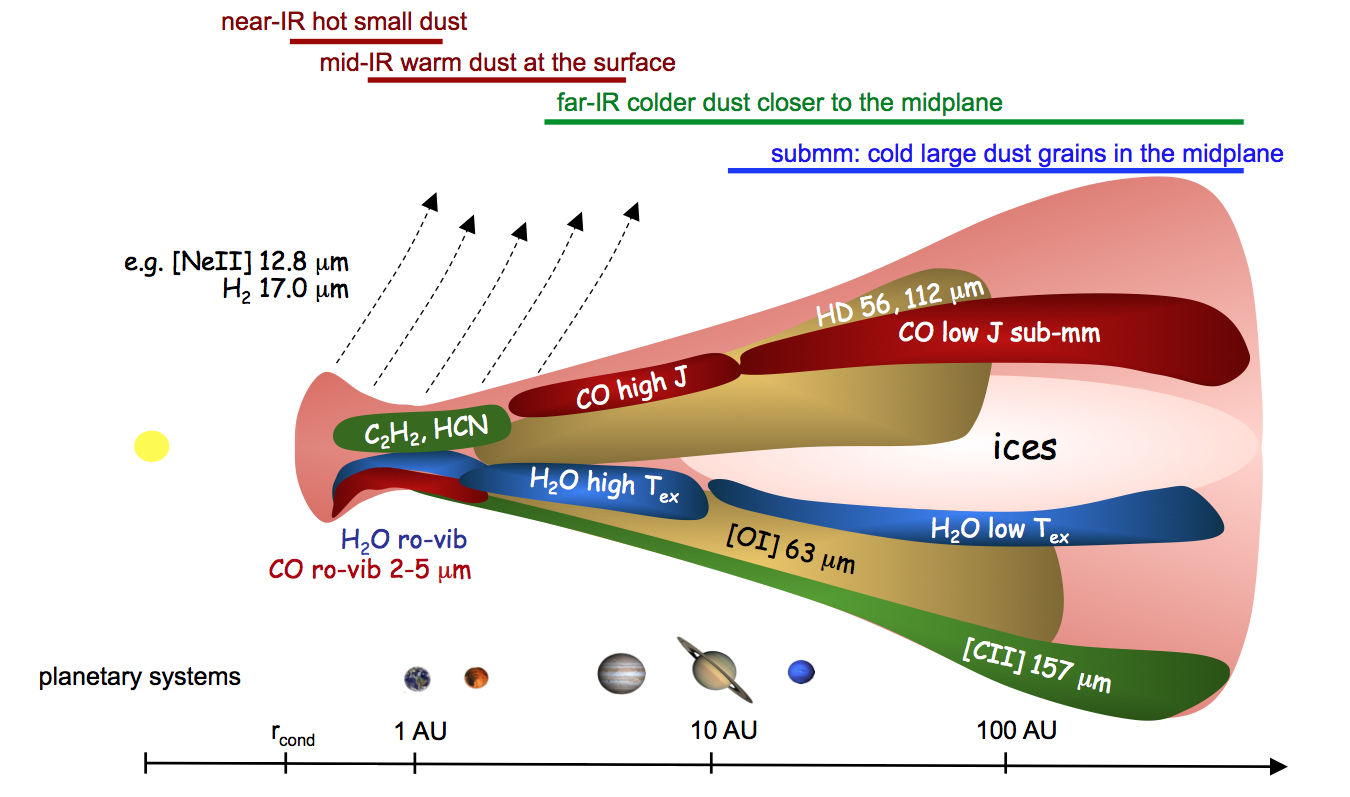
\includegraphics[width=\linewidth]{Figures/disk-sketch.png}
%     \caption{A schematic representation of a protoplanetary disk. The planets in the solar system are shown as a point of reference. \cite{inproceedings}}
%     \label{fig: enter-label}
% \end{figure}

I have mostly worked out the methods and results section. Other than that, I'll put some points i want to include in the other chapters.
\section{Disk Chemistry}
Explaining something about general chemistry, including in-depth nitrogen chemistry

\section{Emission Mechanisms}
It is important to understand how molecules emit photons. In this section, we will explain how these processes work. This is largely based on Chapter 11 of \cite{1979rpa..book.....R}. 

When an electron transitions from an energy state with higher energy to an energy state of lower energy, it emits a photon with a wavelength

\begin{equation}
    \lambda=\frac{hc}{\Delta E}
\end{equation}

where $\Delta E$ is the difference in energy between the two states. 3 different transitions can take place within molecules. 

First, there is the electronic transition. In this transition, an electron jumps from an orbital with higher energy to one with lower. UV 

Second, there is the rotational transition. This transition changes the angular momentum of the molecule.radio and microwave

\begin{equation}
    E^{rot}=B_eK(K+1)
\end{equation}

where J is the rotational quantum number

\begin{equation}
    \Delta  E^{rot}=2B_e(K+1)
\end{equation}

Last, there are ro-vibrational transitions. This changes the vibration and rotation of the molecule. Explain something about PQR branches. IR

\begin{equation}
    E^{vib}=\hbar\omega(v+1)
\end{equation}
with $\omega=\sqrt{\frac{k}{\mu}}$ and $v$ the vibrational quantum number.
\begin{equation}
    \Delta E^{vib}=\hbar\omega
\end{equation}

selection rules:
$\Delta v=\pm 1; \Delta K = 0, \pm1 (and for some \Delta K=0 is forbidden)$

\section{JWST MIRI MRS}


\section{Modeling}
% Some of the properties of the protoplanetary disks can be directly inferred from disk measurements. For instances where this is not the case, we would still like to learn more from our data via a different method. We can use models to simulate the protoplanetary disk and generate synthetic data to compare to actual observations. There are various types of models. Ranging from 1D slab models to thermo-chemical disk models. For our research, we run simulations using the PROtoplanetary Disk Model (ProDiMo), a thermo-chemical disk model. The output of those simulations is then put through Fast Line Tracing system (FLiTs) to get an accurate spectrum of the disk. 

\section{Goal}
We want to search for a method to detect NO and NH\3 in the spectra of protoplanetary disks using JWST MIRI MRS. 
We present the methodology in chapter \ref{Ch: Methods}. The data and results are shown in chapter \ref{Ch: Results}. We discuss the results and their implications in chapter \ref{Ch: Discussion}. In chapter \ref{Ch: Conclusion}, we conclude our thesis.
\chapter{Methods}\label{Ch: Methods}
\section{ProDiMo Simulations}

\begin{table}[!ht]
\centering
\begin{tabular}{@{}lll@{}}
                                  &                             &                            \\ \hline\midrule
\textbf{Property}                 & \textbf{Symbol}             & \textbf{Value}             \\ \midrule
Stellar mass                      & M$_\ast$                    & 0.7M$_\odot$               \\
Effective Temperature             & T$_\ast$                    & 4000 K                     \\
Stellar Luminosity                & L$_\ast$                    & 1 L$_\odot$                \\
UV excess                         & f$_{UV}$                    & 0.01                       \\
UV powerlaw index                 & p$_{UV}$                    & 1.3                        \\
X-ray luminosity                  & L$_x$                       & 10$^30$ erg/s              \\
X-ray emission temperature        & T$_x$                       & 2$\times10^7$ K            \\ \midrule
Strength of interstellar UV       & $\chi^{ISM}$                & 1                          \\
Strength of interstellar IR       & $\chi^{ISM}_{IR}$           & 0                          \\
Cosmic ray H$_2$ ionization rate & $\zeta_{CR}$                & $1.7\times10^{-17} s^{-1}$ \\ \midrule
Inner disk radius                 & R$_{in}$                    & 0.05 au                    \\
Outer disk radius                 & R$_{tap}$                   & 30 au                      \\
Column density power index        & $\epsilon$                  & 1                          \\
Reference scale height            & H$_g$ (100 au)              & 10 au                      \\
Flaring power index               & $\beta$                     & 1.15                       \\ \midrule
Minimum dust particle radius      & a$_{min}$                   & 0.05 $\mu$m                \\
Maximum dust particle radius      & a$_{max}$                   & 3000 $\mu$m                \\
Dust size dist. power index       & a$_{pow}$                   & 3.5                        \\
Turbulent mixing parameter        & $\alpha_{settle}$           & 0.001                      \\
Refractory dust composition       & Mg$_{0.7}$Fe$_{0.3}$SiO\3 & 60 \%                      \\
                                  & amorph. C                   & 15 \%                      \\
                                  & porosity                    & 25 \%                      \\
PAH abundance rel. to ISM         & f$_{PAH}$                   & 0.01                       \\
Chemical heating efficiency       & $\gamma^{chem}$             & 0.2                        \\ \midrule
Distance to the observer          & d                           & 140 pc                     \\ \bottomrule
\end{tabular}
\caption{Disk parameters used for the models}
\label{tab: parameters}
\end{table}
To investigate whether we can detect NO and NH\3 in the spectra of protoplanetary disks and how nitrogen carriers depend on the C and O abundance, 
we ran a model grid with varying abundances of C and O using ProDiMo. The parameters with which the models were run are in \autoref{tab: parameters}. 
\begin{equation}
    \epsilon_X\equiv\log\frac{N_X}{N_H}+12
\label{eq: abundance}
\end{equation}
The abundances are defined as in \autoref{eq: abundance}. In this system $\epsilon_H=12$. 
The abundances of C and O were varied between -0.5 and 0.5 in steps of 0.25, where 0 corresponds to the solar abundance. The grid contains 25 models, with the fiducial model in the middle, which is based on the solar abundances of C and O. Furthermore, we increased the nitrogen abundance by an order of magnitude compared to the solar abundance.

\begin{table}[!ht]
\centering
\begin{tabular}{@{}lll@{}}
                                  &                             &                            \\ \hline\midrule
\textbf{Element} & \textbf{+12 Abundance} & \textbf{Variation}            \\ \midrule
H                & 12                     & Fixed                         \\
He               & 10.984                 & Fixed                         \\
C                & 8.140                  & {[}-0.5, -0.25, 0, +0.25, +0.5{]} \\
N                & 8.900                  & Fixed                         \\
O                & 8.480                  & {[}-0.5, -0.25, 0, +0.25, +0.5{]} \\
Ne               & 7.950                  & Fixed                         \\
Na               & 3.360                  & Fixed                         \\
Mg               & 4.030                  & Fixed                         \\
Si               & 4.240                  & Fixed                         \\
S                & 5.270                  & Fixed                         \\
Ar               & 6.080                  & Fixed                         \\
Fe               & 3.240                  & Fixed                         \\
PAH              & 3.444                  & Fixed                         \\ \bottomrule
\end{tabular}
\caption{The elemental abundances used in the simulation of the model grid}
\label{tab: abundances}
\end{table}



After running the model grid, we used FLiTs to generate the spectra for all the models. We calculated the entire spectrum containing  \textbf{INSERT EXACT MOLECULES IN THE TOTAL SPECTRUM} and the spectra of individual molecules as well. The spectra we retrieved with FLiTs have an unrealistically high resolution. To make the spectrum more realistic, we convolved the spectrum to a resolving power of $R = \Delta\lambda/\lambda = 3000$ using a Gaussian kernel to create a spectrum of the correct resolving power. The value of 3000 was chosen as it is approximately the average resolving power of the MIRI MRS \citep{SOURCE}. 

We wanted to add noise to the data to make the simulated spectra as realistic as possible. The MINDS team has observations which have $SNR = 300$ \citep{SOURCE}. We want to make our simulated data follow the same vein. We estimate the noise level needed to create an $SNR = 300$ using the spectrum minimum before continuum subtraction. We assume that the noise is normally distributed. After applying this noise, we subtract the continuum to get the spectrum we can use to analyze the different molecules that compose it.


The flux density we have from FLiTs is in units of Jansky, but we would like to integrate the flux density to get the flux. For this, we need to convert the flux per unit frequency to flux per unit wavelength. We use the equation

\begin{equation}
    F_\lambda=\frac{c}{\lambda^2}F_\nu
\end{equation}

\textbf{SPECTRUM CLASSIFICATION}
The different species have different spectral regions in which they emit. To classify these regions, we split the entire spectrum into windows of 0.001 $\mu$m from 4.9 to 27.5 $\mu$m. Next, we integrate the spectrum for each species in that window and store the species that has the highest flux in that region. Doing this for all models and taking the mode. We get the species for each window that has the strongest emission for most of the simulated spectra.  


\section{Cross-Correlation}
For our analysis, we used cross-correlation. This is a signal detection technique for detecting weak signals. We implemented this to detect the weak spectral features of NO and NH\3 It is defined as follows. 
\begin{equation}
    R_{fg}(\tau)=\int^\infty_{-\infty}\overline{f(t)}g(t+\tau)dt
\end{equation}
The autocorrelation is the cross-correlation of a function with itself
\begin{equation}
    R_{ff}(\tau)=\int^\infty_{-\infty}\overline{f(t)}f(t+\tau)dt
\end{equation}
As all our functions are real valued, we can omit the complex conjugation in the integrand.

We calculated the average spectrum for each species and divided that by the maximum of the spectrum to normalize it. We used this template spectrum to cross-correlate with the spectrum containing all the species. The cross-correlation should peak when the template spectrum matches the spectrum containing all the species. To quantify the height of the peak, we calculated the difference between the height of the peak and the median value of the cross-correlation in a small region around the peak. We took the median as this is less susceptible to outliers to capture the general trend around the peak more optimally. We used hypothesis testing to test whether or not there is statistical evidence to say the molecule is present. We had the following null hypothesis and alternative hypothesis

\begin{equation}
    H_0: \text{The height of the peak in the cross-correlation is caused by noise}
\end{equation}
\begin{equation}
    H_1: \text{The height of the peak in the cross-correlation is caused by the molecule}
\end{equation}

To assess the significance of the peak in cross-correlation, we used a Monte Carlo simulation to simulate 10000 synthetic spectra under the null hypothesis. First, we take all the flux values we have for different wavelength values. Second, we sample with replacement from the flux values until we have a collection of values that is the same size as the original set. Third, we take the cross-correlation and calculate the difference between the height of the peak and the median value of the cross-correlation in a small region around the peak. The value of the original data is deemed significant when it exceeds 95\% of the values from the simulated data ($\alpha=0.05$)


\section{Observations}
After looking at the simulated spectra, we wanted to apply our techniques to observations made with JWST MIRI MRS. We have access to 3 sources. 

\textbf{MASKING OF REGIONS}
LTE models to fit the model and try to enhance the hidden molecules
\textbf{MORE EXPLANATION NEEDED}
\begin{figure}[!ht]
    \centering
    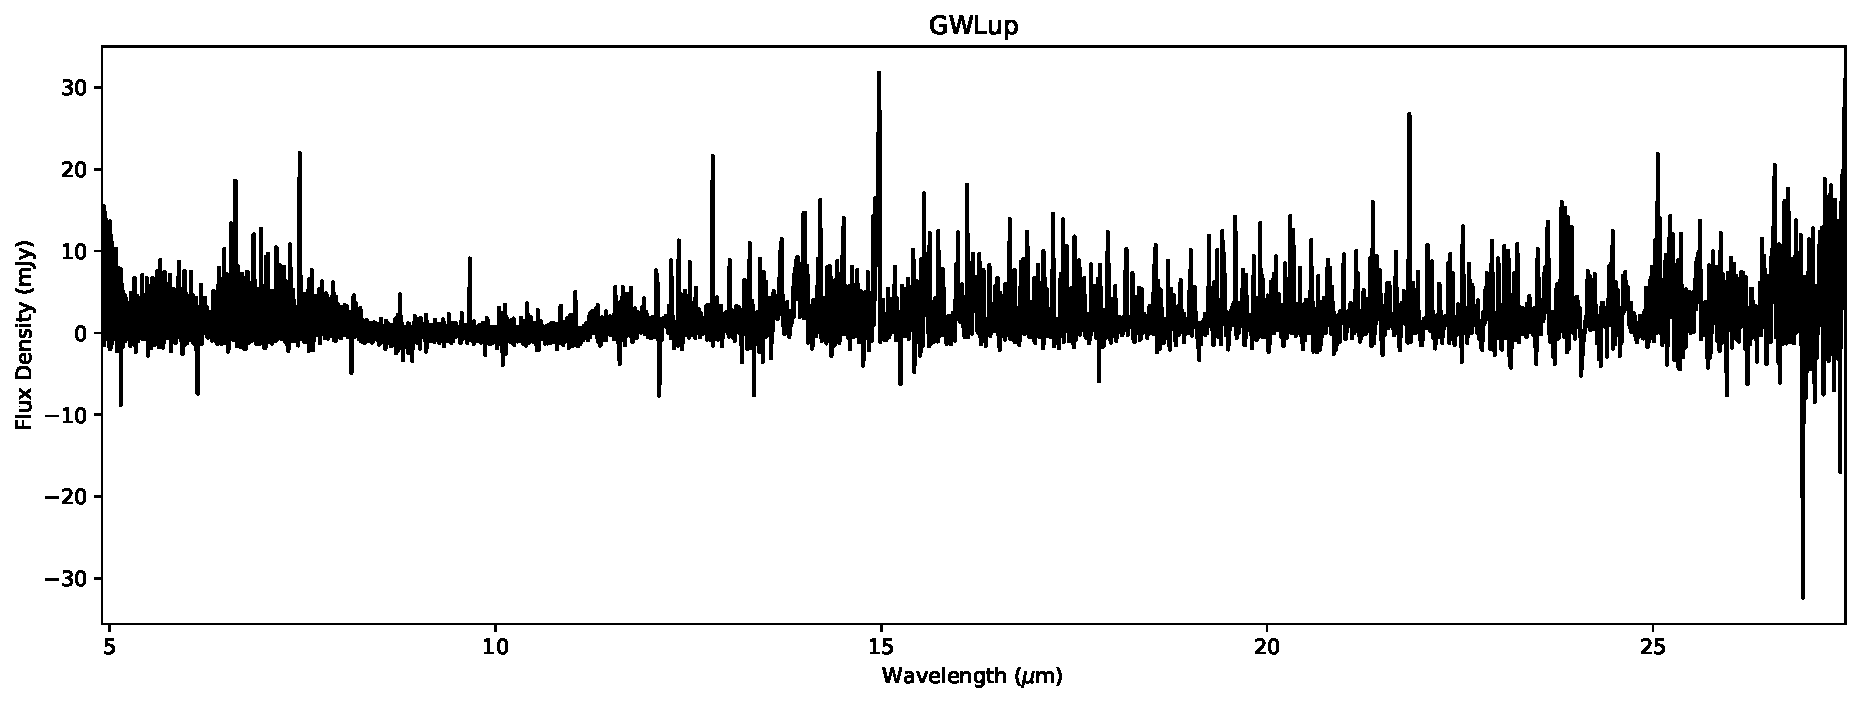
\includegraphics[width=\linewidth]{Figures/FullSpectrum_GWLup.pdf}
    \caption{The continuum subtracted spectrum of GWLup}
    \label{fig: GWLup}
\end{figure}
\begin{figure}[!ht]
    \centering
    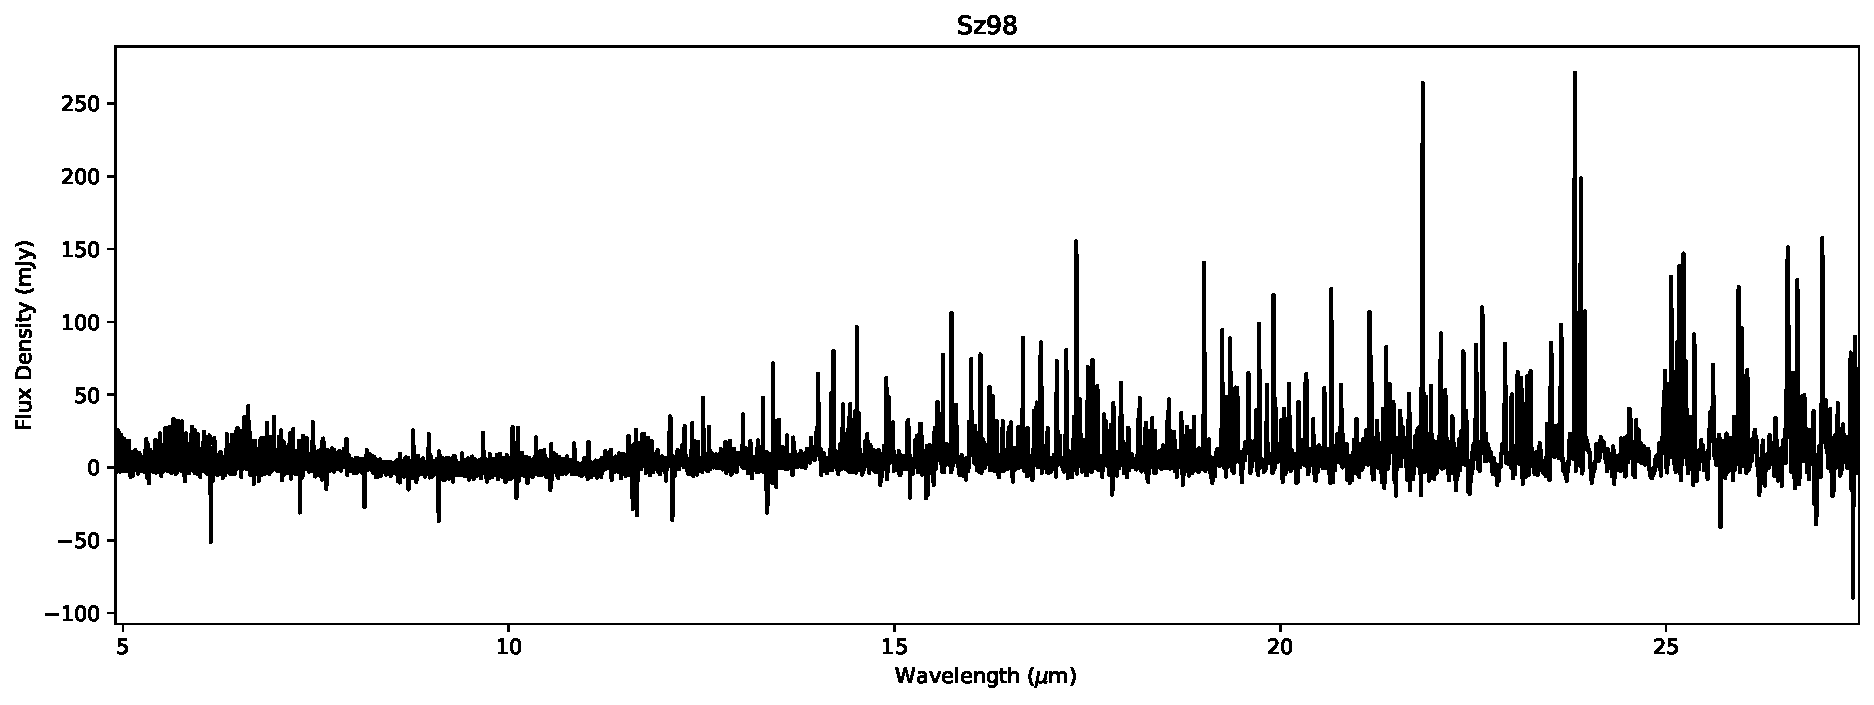
\includegraphics[width=\linewidth]{Figures/FullSpectrum_Sz98.pdf}
    \caption{The continuum subtracted spectrum of Sz98}
    \label{fig: Sz98}
\end{figure}
\begin{figure}[!ht]
    \centering
    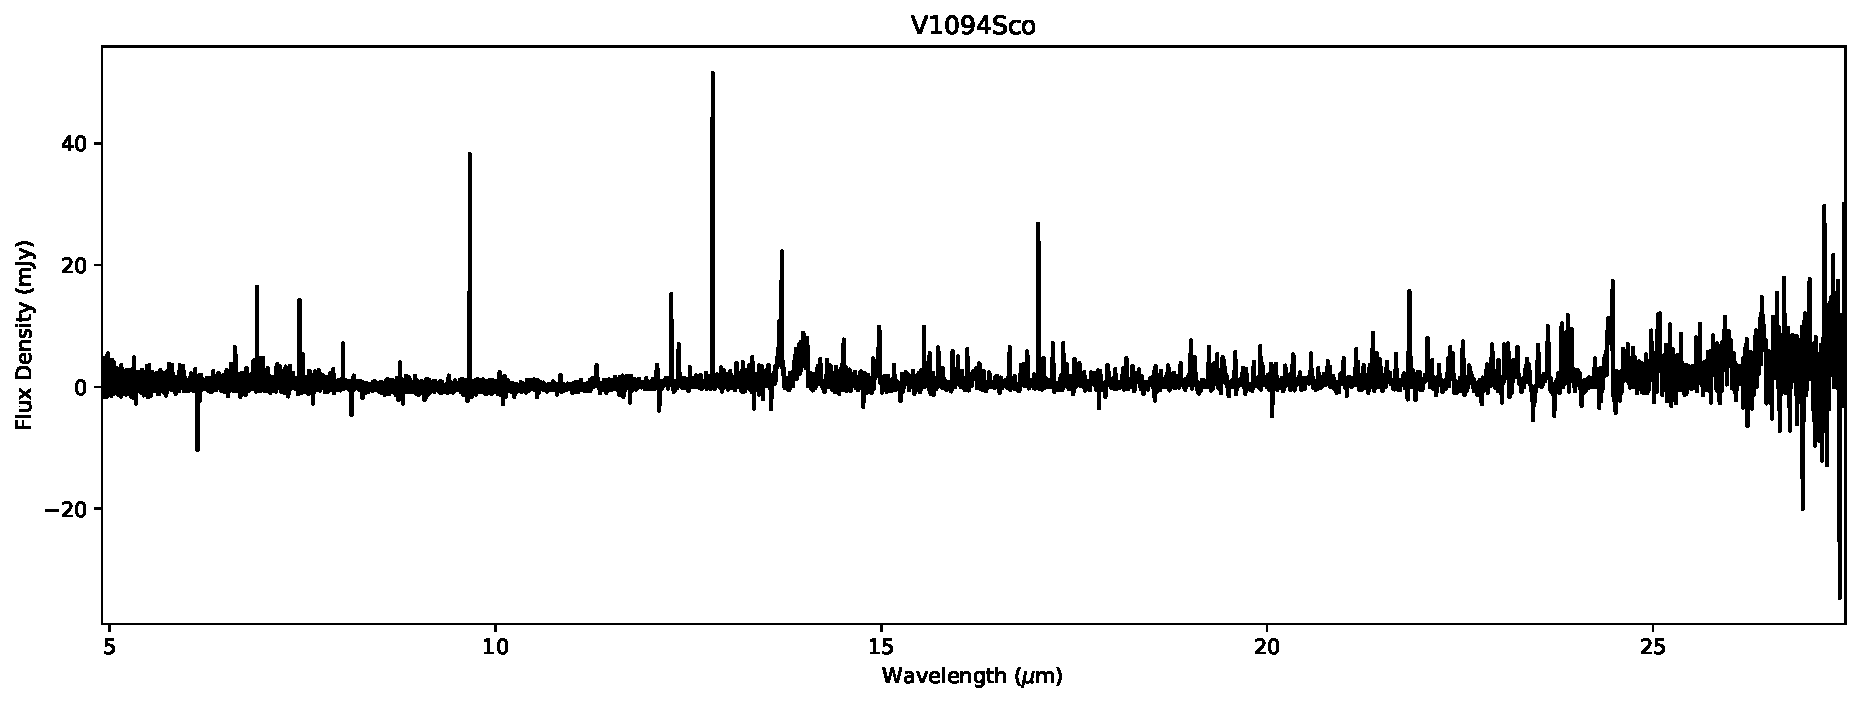
\includegraphics[width=\linewidth]{Figures/FullSpectrum_V1094Sco.pdf}
    \caption{The continuum subtracted spectrum of V1094Sco}
    \label{fig: V1094Sco}
\end{figure}



\chapter{Results}\label{Ch: Results}
\section{ProDiMo Output}
After running the models, we analyzed their output. First, we looked at the densities of the gas and dust in the disk. The densities of the fiducial model are shown in \autoref{fig: density}. The density of the gas is more vertically extended than the density of the dust. This is expected, as we know that the dust settles around the midplane. Furthermore, the density of the gas stretches further from the host star than the dust.

\begin{figure}[!ht]
    \centering
    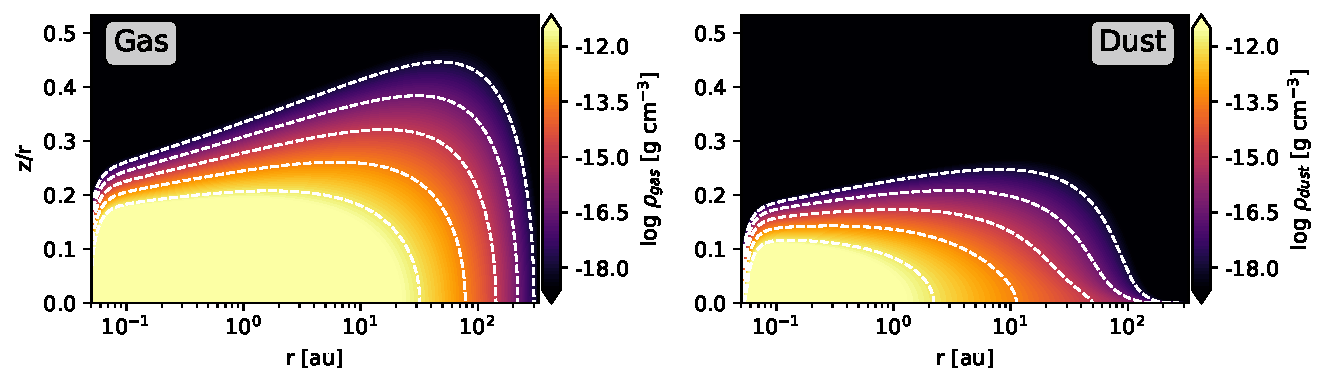
\includegraphics[width=\linewidth]{Figures/Density.pdf}
    \caption{The distribution of gas and dust in the disk of the fiducial model.}
    \label{fig: density}
\end{figure}

Subsequently, we inspected the temperatures of gas and dust across the disk. Those are shown in \autoref{fig: temperature}.  The gas and dust temperatures vary across the disk for different heights and radii. However, they are equal in the midplane as they are coupled. Above the midplane, they decouple, and the gas and dust temperatures change. The gas temperatures are higher as they get heated by the star, whereas the dust temperatures are lower. Notably, the temperature gradient of the dust is vertically isothermal. This result is expected as the density of the dust is orders of magnitude lower in the regions above the disk. This results in the starlight getting barely blocked, so the temperature doesn't change across different heights.

\begin{figure}[!ht]
    \centering
    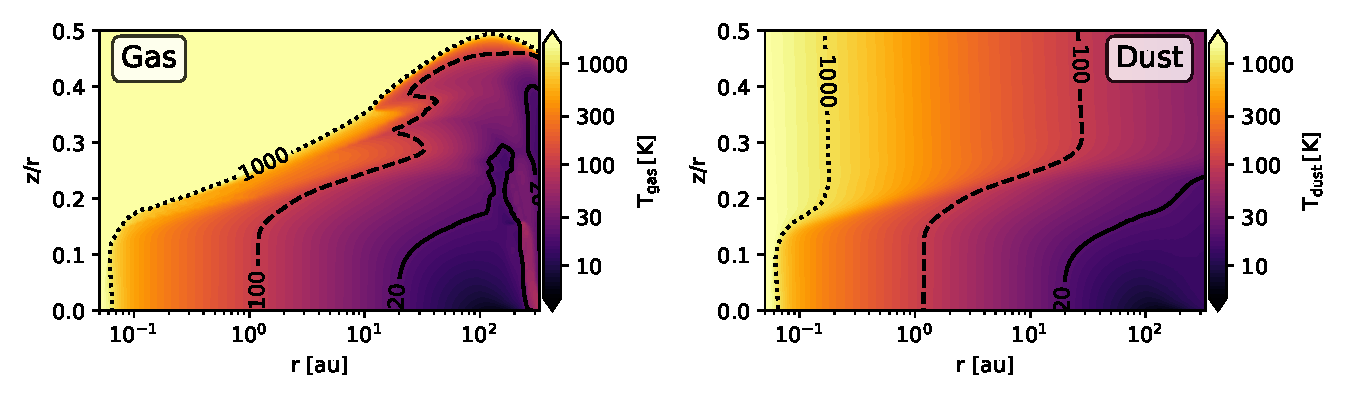
\includegraphics[width=\linewidth]{Figures/Temperature.pdf}
    \caption{The temperature profile of gas and dust in the disk of the fiducial model.}
    \label{fig: temperature}
\end{figure}

Lastly, we inspected the distribution of nitrogen-bearing molecules: HCN, HNC, NH\3, and NO. Figure \ref{fig: nitrogen distribution} shows their distribution. The density of the molecules changes a lot for different radii and heights. For example, in the region between 0.05 and 0.1 au we see that HCN decreases compared to the surrounding regions, but HNC increases in the same region. There is a gap in the densities between 1 and 200 au. In these regions, the temperature drops below the freezing point of these molecules, resulting in the formation of ice. 

\begin{figure}[!ht]
    \centering
    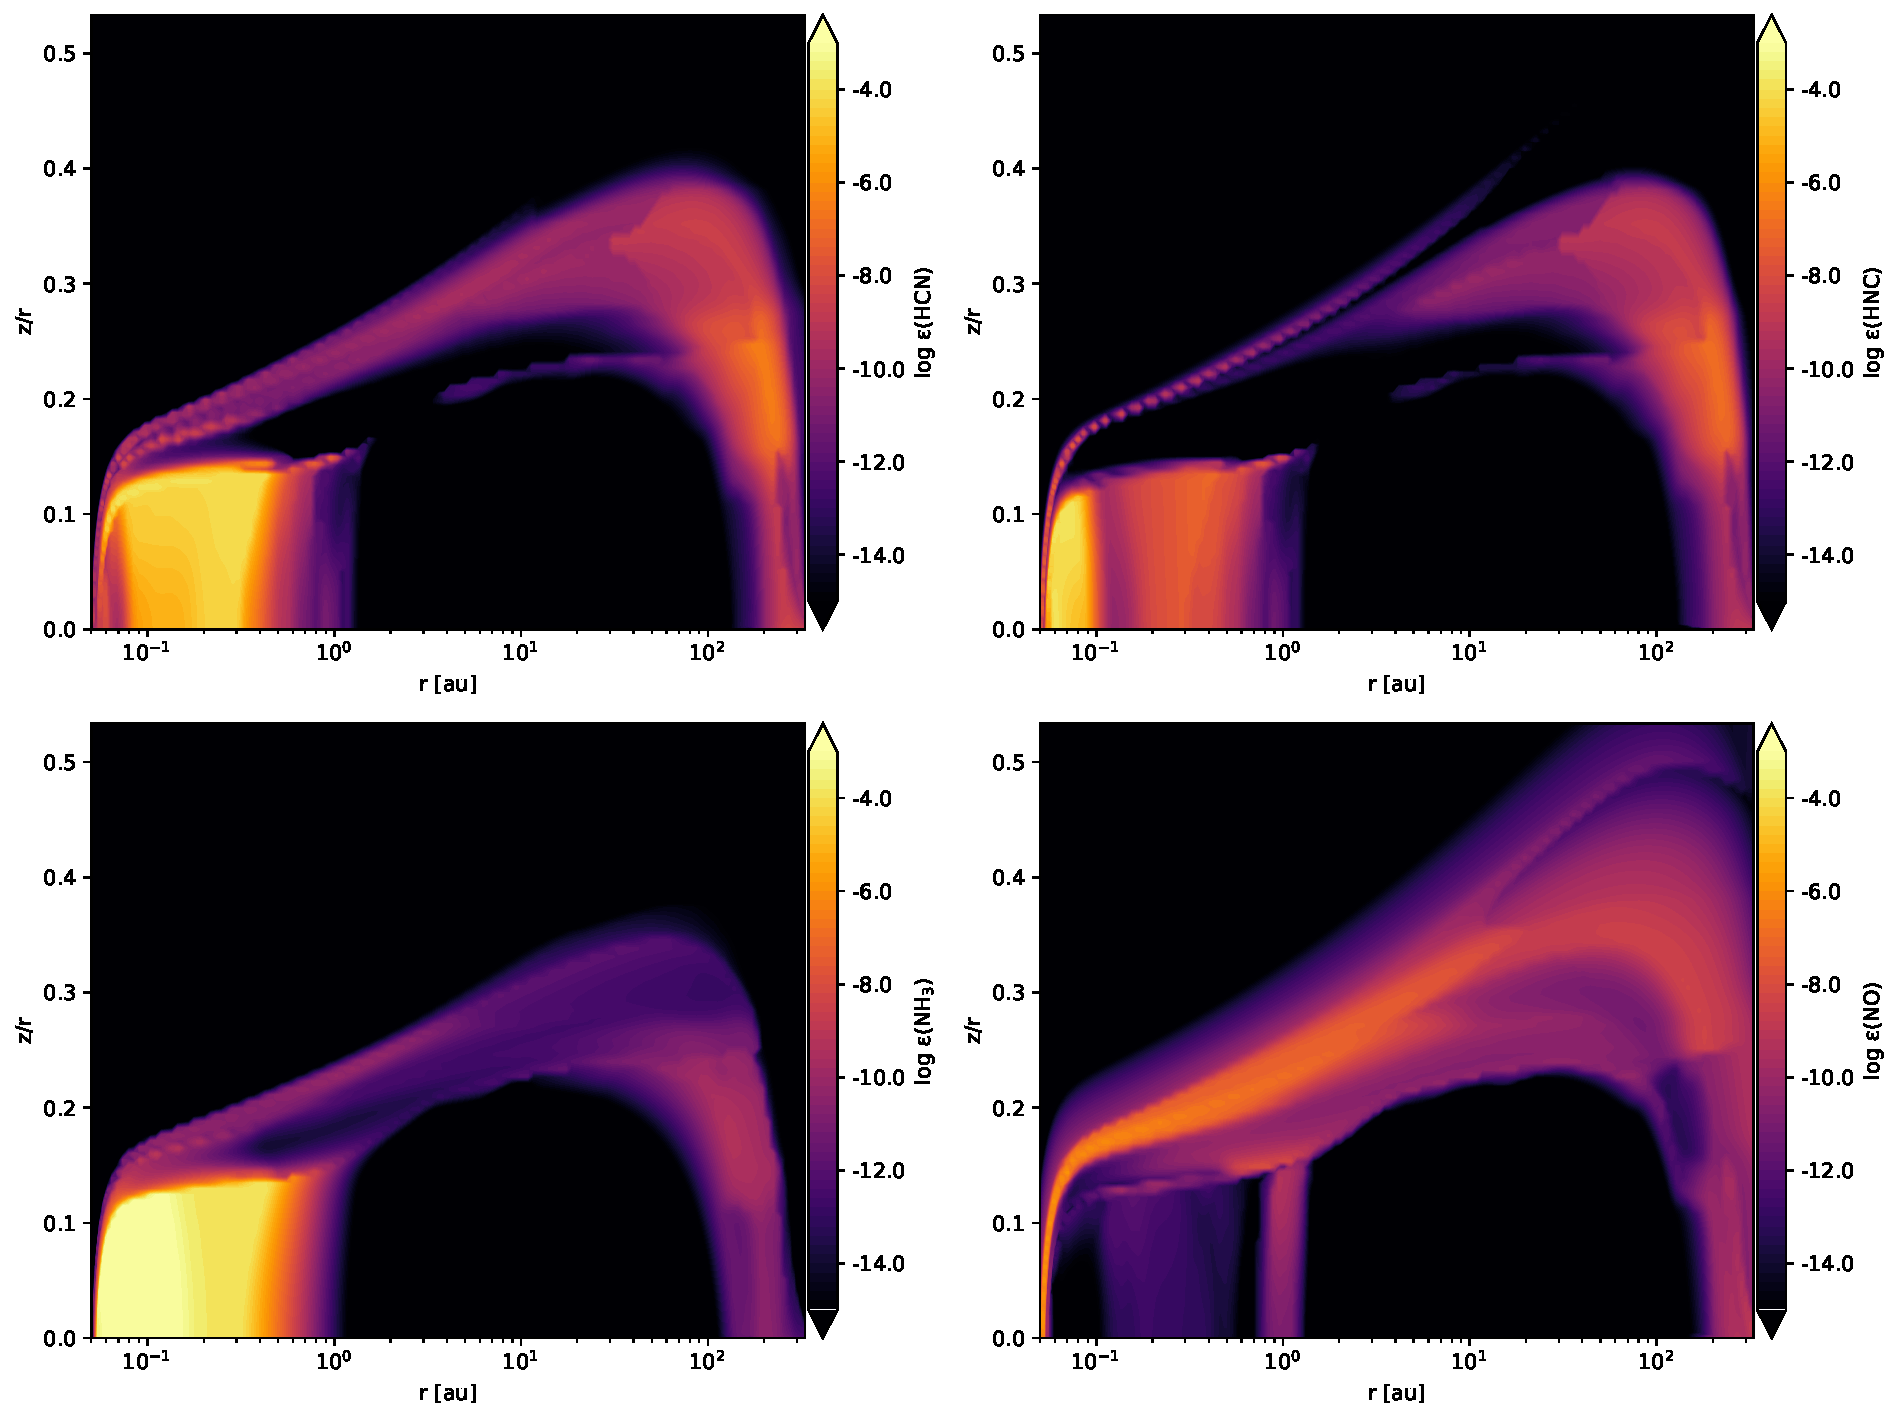
\includegraphics[width=.8\linewidth]{Figures/Abundance.pdf}
    \caption{The distribution of HCN, HNC, NH\3, and NO across the disk of the fiducial model.}
    \label{fig: nitrogen distribution}
\end{figure}

\section{FLiTs Spectra}
The models in the model grid we created were used with FLiTs to create accurate spectra. The resulting spectra are shown in figure \ref{fig: all spectra}. There is a clear division in the shapes of the spectra. In the bottom left corner, you have 6 spectra that have a strong HCN feature. These models also have a C/O ratio greater than unity. The other models have strong water features and have a C/O ratio smaller than unity. 

\begin{figure}[!ht]
    \centering
    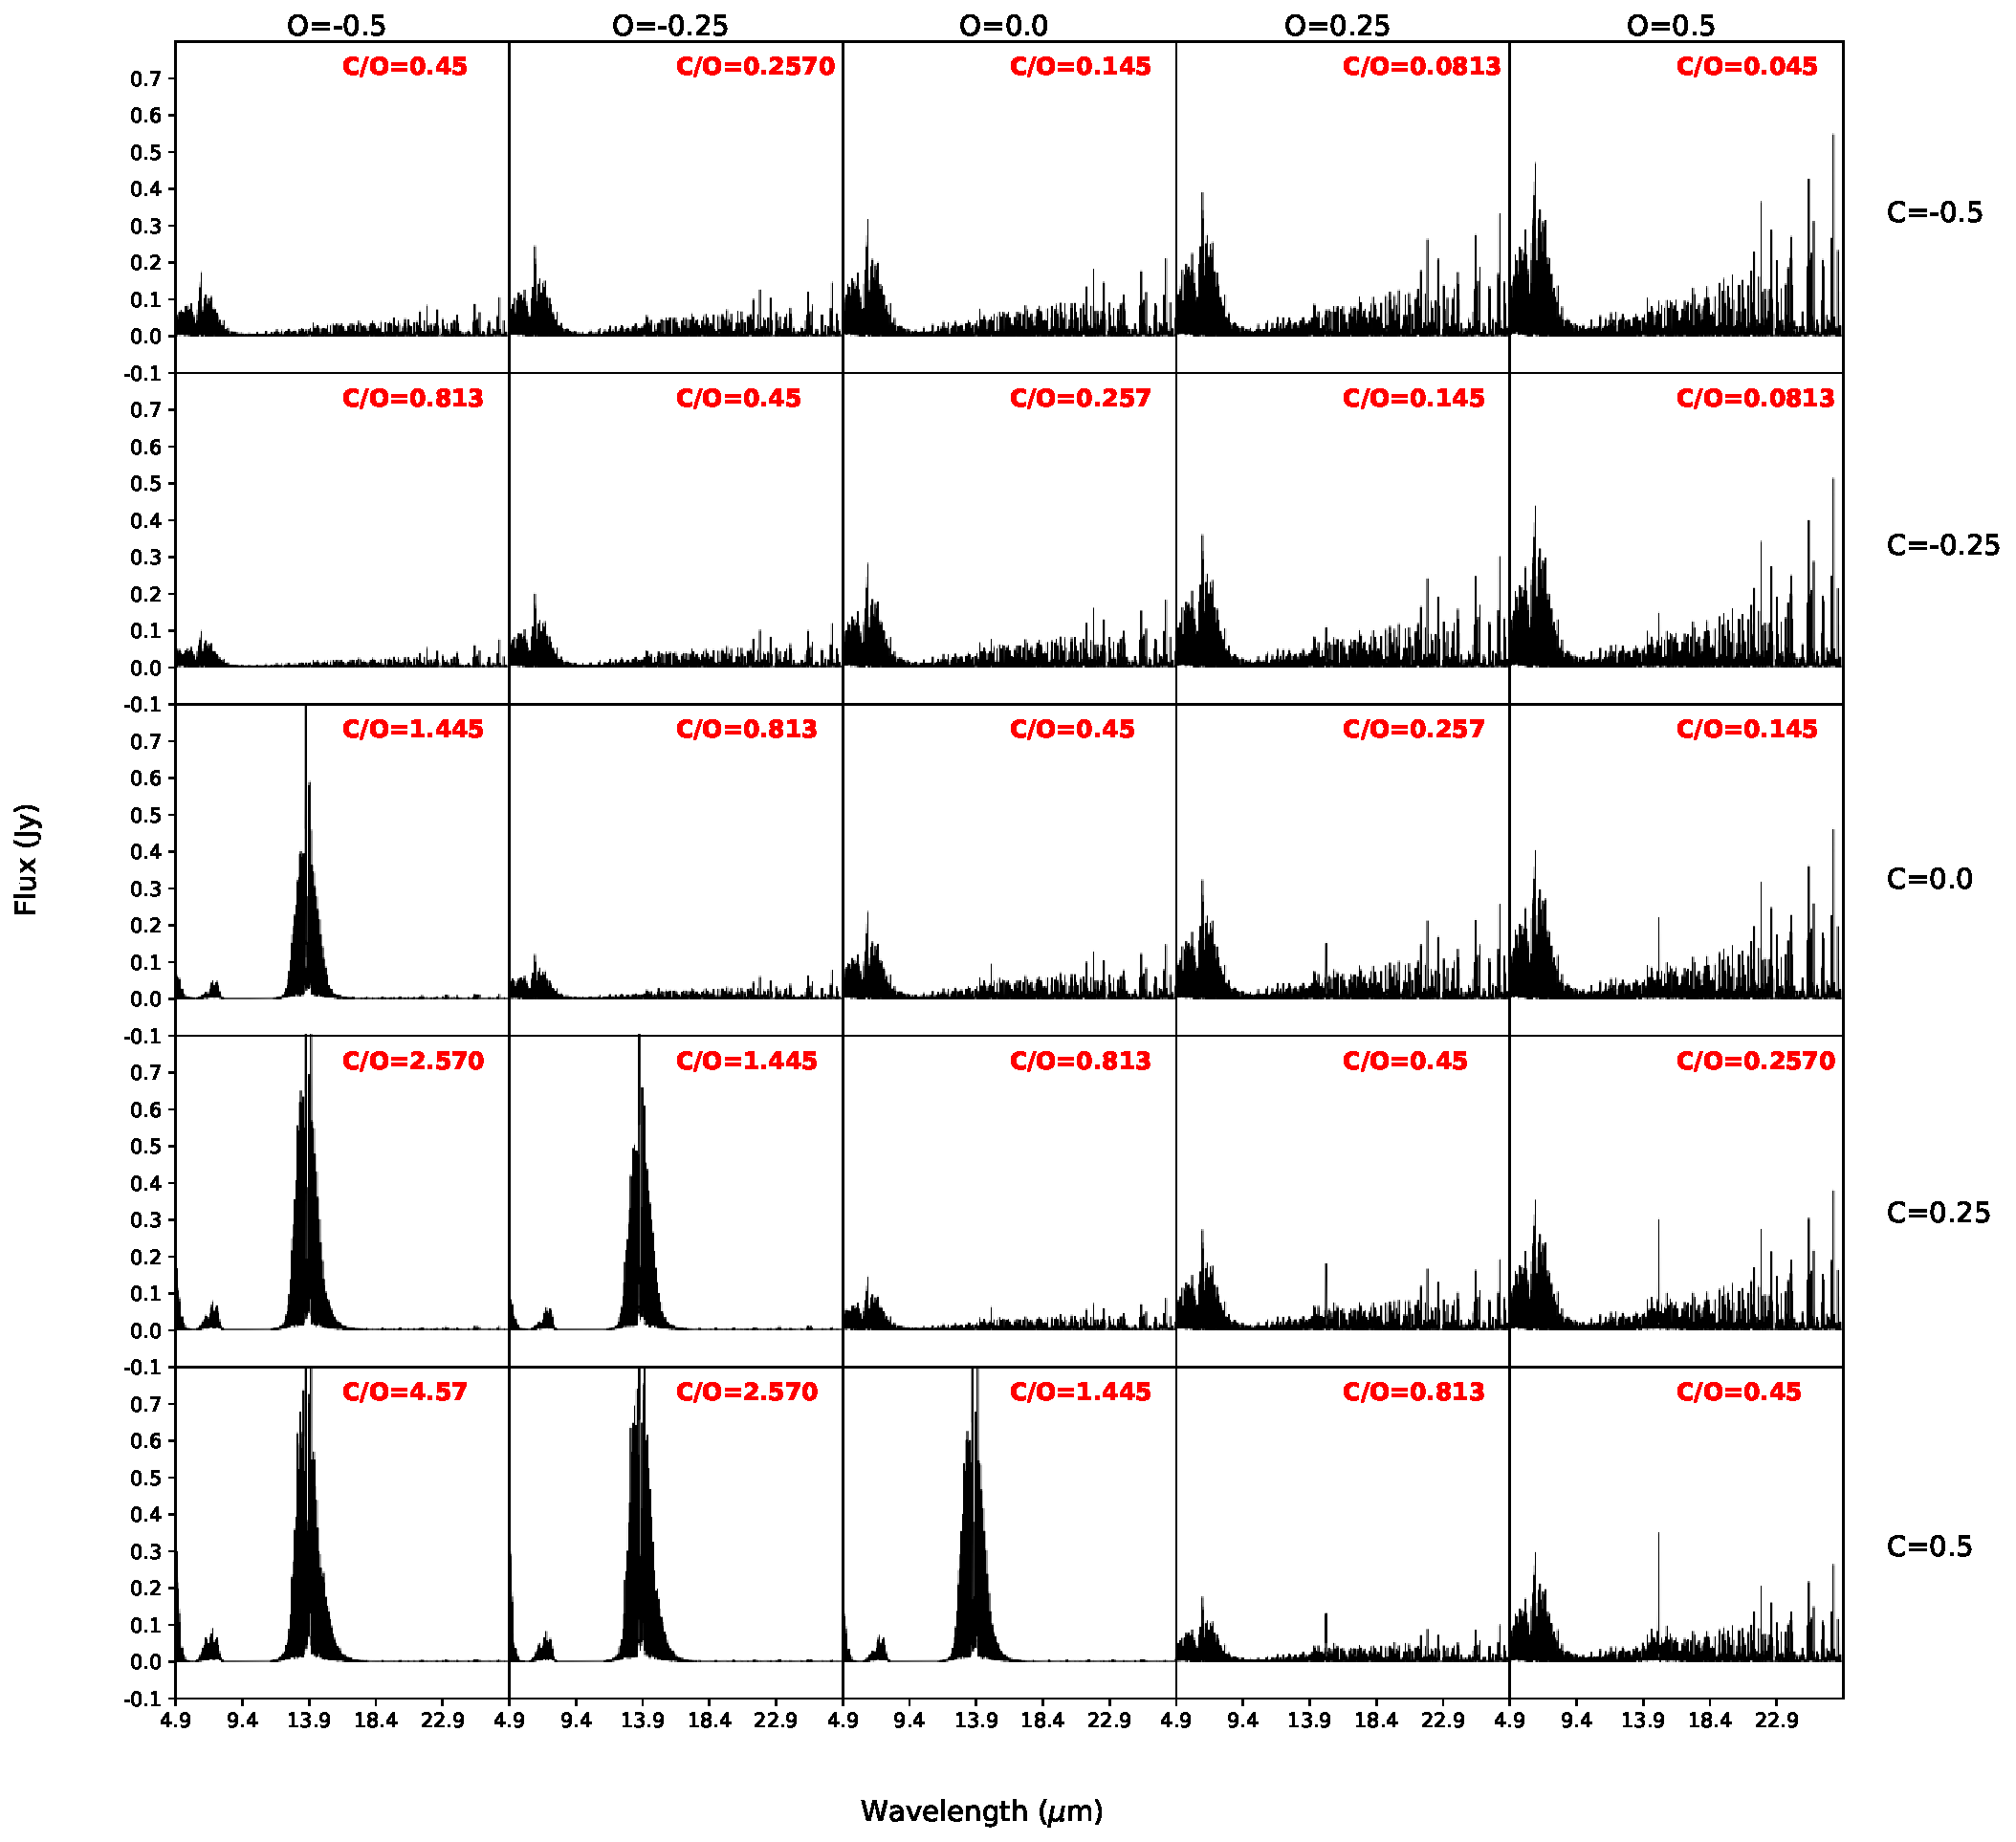
\includegraphics[width=\linewidth]{Figures/All_spectra.pdf}
    \caption{The simulated spectra of all the models in the model grid using FLiTs. On the horizontal axis, the O abundance is varied from -0.5 to 0.5 w.r.t. the reference abundance. The C abundance is varied with -0.5 to 0.5 w.r.t. the reference abundance from top to bottom.}
    \label{fig: all spectra}
\end{figure}

The flux of the different species changes depending on the abundances of C and O. The total flux for HCN, NO, and NH\3 for all the models in the model grid are shown in figures \ref{fig: flux HCN}, \ref{fig: flux NO}, and \ref{fig: flux NH3}. 

\begin{figure}[!ht]
    \centering
    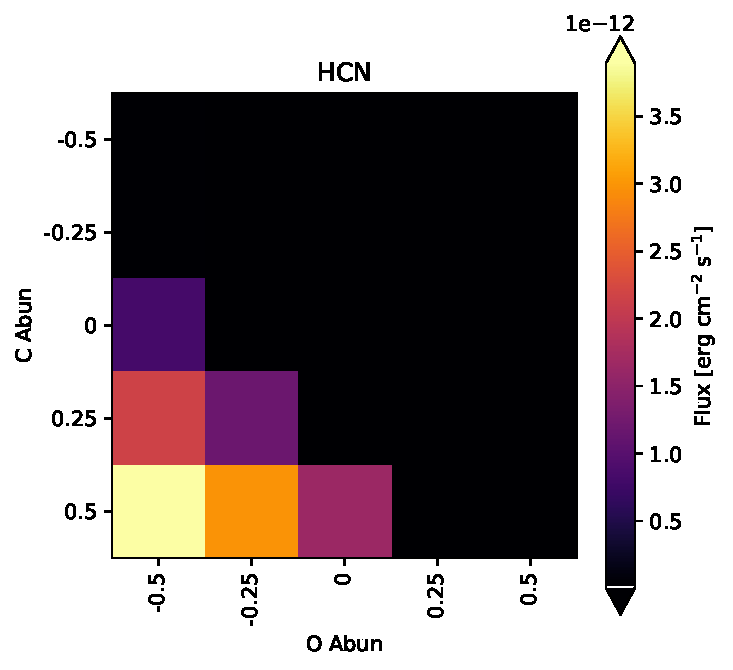
\includegraphics[width=0.5\linewidth]{Figures/HCN_heatmap.pdf}
    \caption{The total flux of HCN for all the models in the grid.}
    \label{fig: flux HCN}
\end{figure}

\begin{figure}[!ht]
    \centering
    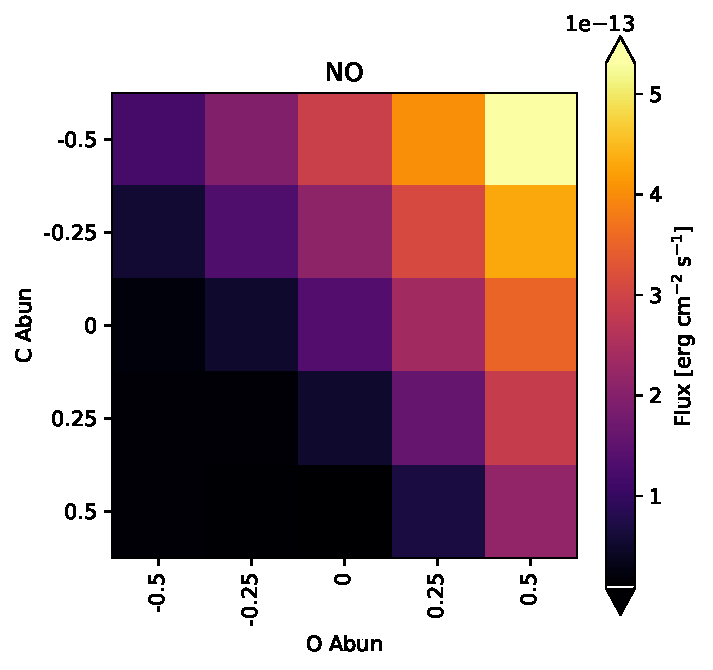
\includegraphics[width=0.5\linewidth]{Figures/NO_heatmap.pdf}
    \caption{The total flux of NO for all the models in the grid.}
    \label{fig: flux NO}
\end{figure}

\begin{figure}[!ht]
    \centering
    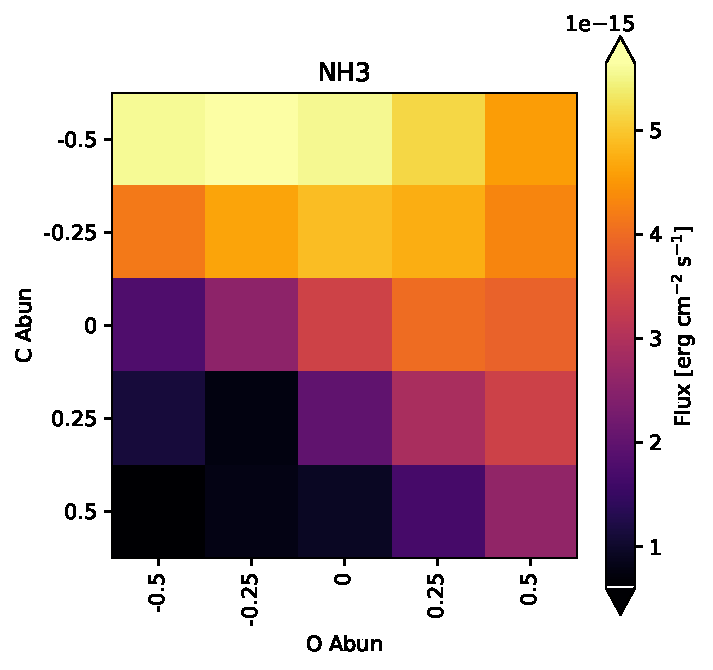
\includegraphics[width=0.5\linewidth]{Figures/NH3_heatmap.pdf}
    \caption{The total flux of NH\3 for all the models in the grid.}
    \label{fig: flux NH3}
\end{figure}

The HCN increases as C/O gets larger, and NO decreases with it. The flux of NH\3 generally increases as the C abundance gets lower. We hypothesize that the reason for this is the reactions that take place to form NH\3.
We believe that OH is an important component in the formation of NH\3.

\ce{NH2+ + OH -> NH3 + O+}

\textbf{MORE REACTIONS}

Next, we wanted to identify regions in the spectrum that could help us detect NO and NH\3. We split the model grid into 2 groups. One group has C/O smaller than unity, and the other greater. We chose this distinction as the behaviors of the spectra are different. This difference is also visible in figure \ref{fig: all spectra}. 

\begin{figure}[!ht]
    \centering
    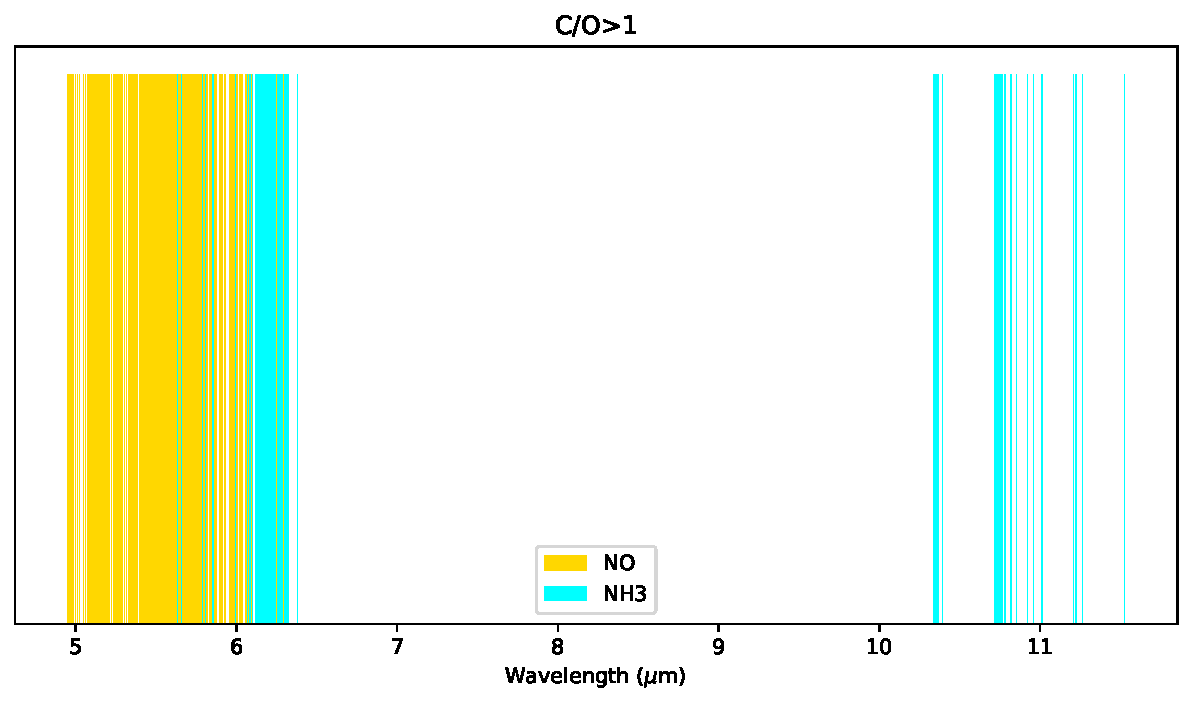
\includegraphics[width=\linewidth]{Figures/ClassificationCOgt0.pdf}
    \caption{The regions of the spectrum where NO and NH\3 emission are the  strongest compared to other molecular emission in the models that have a C/O greater than unity}
    \label{fig: class>1}
\end{figure}

\begin{figure}[!ht]
    \centering
    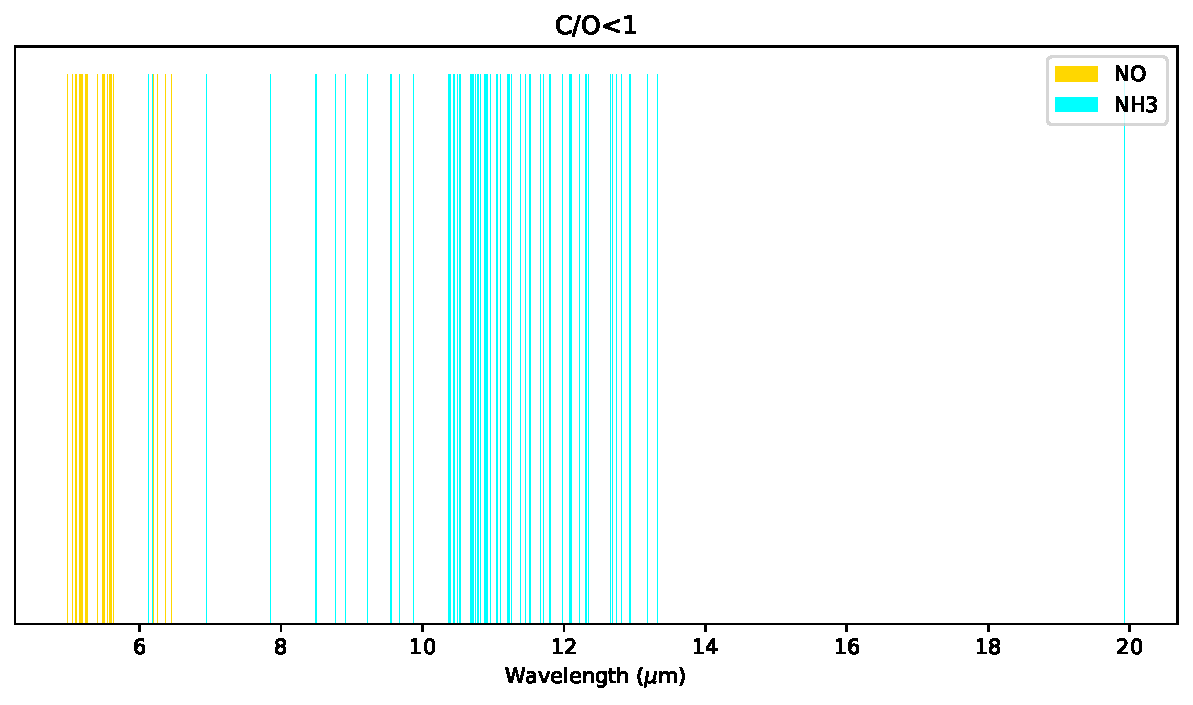
\includegraphics[width=\linewidth]{Figures/ClassificationCOst0.pdf}
    \caption{The regions of the spectrum where NO and NH\3 emission are strongest in the models that have a C/O smaller than unity}
    \label{fig: class<1}
\end{figure}

In figure \ref{fig: class>1}, it is visible that the region between 4.9$\mu$m and 6 $\mu$m has many regions where NO emission is strongest. This coincides with the region where NO has a spectral feature. NH\3 is the brightest between 6 $\mu$m and 6.4 $\mu$m. Between 10 $\mu$m and 12 $\mu$m there are some smaller regions where NH\3 is strongest. In contrast, in figure \ref{fig: class<1}, the regions where NO or NH\3 emission is strongest are more barren. The NO emission regions are not the strongest anymore, as well as the NH\3 emission region next to it. The most promising region for NH\3 is now between 10 $\mu$m and 12 $\mu$m. 

\begin{figure}[!ht]
    \centering
    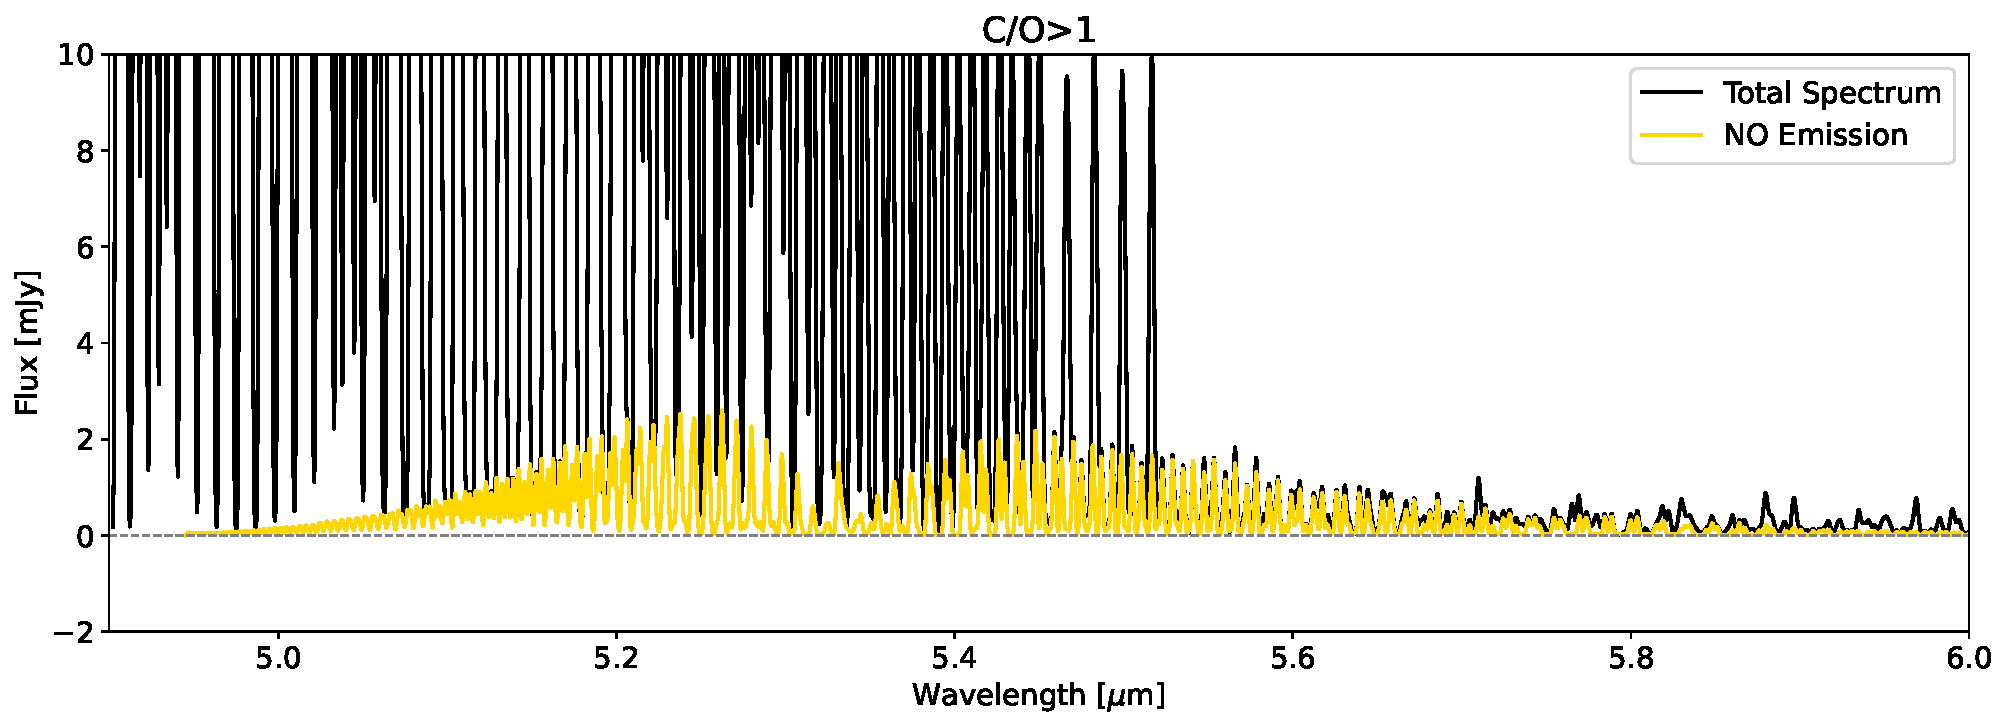
\includegraphics[width=\linewidth]{Figures/NO_region.pdf}
    \caption{A zoomed-in region of the spectrum of the fiducial model between 4.9 $\mu$m and 6 $\mu$m where NO emission is strongest.}
    \label{fig: NO region}
\end{figure}

\begin{figure}[!ht]
    \centering
    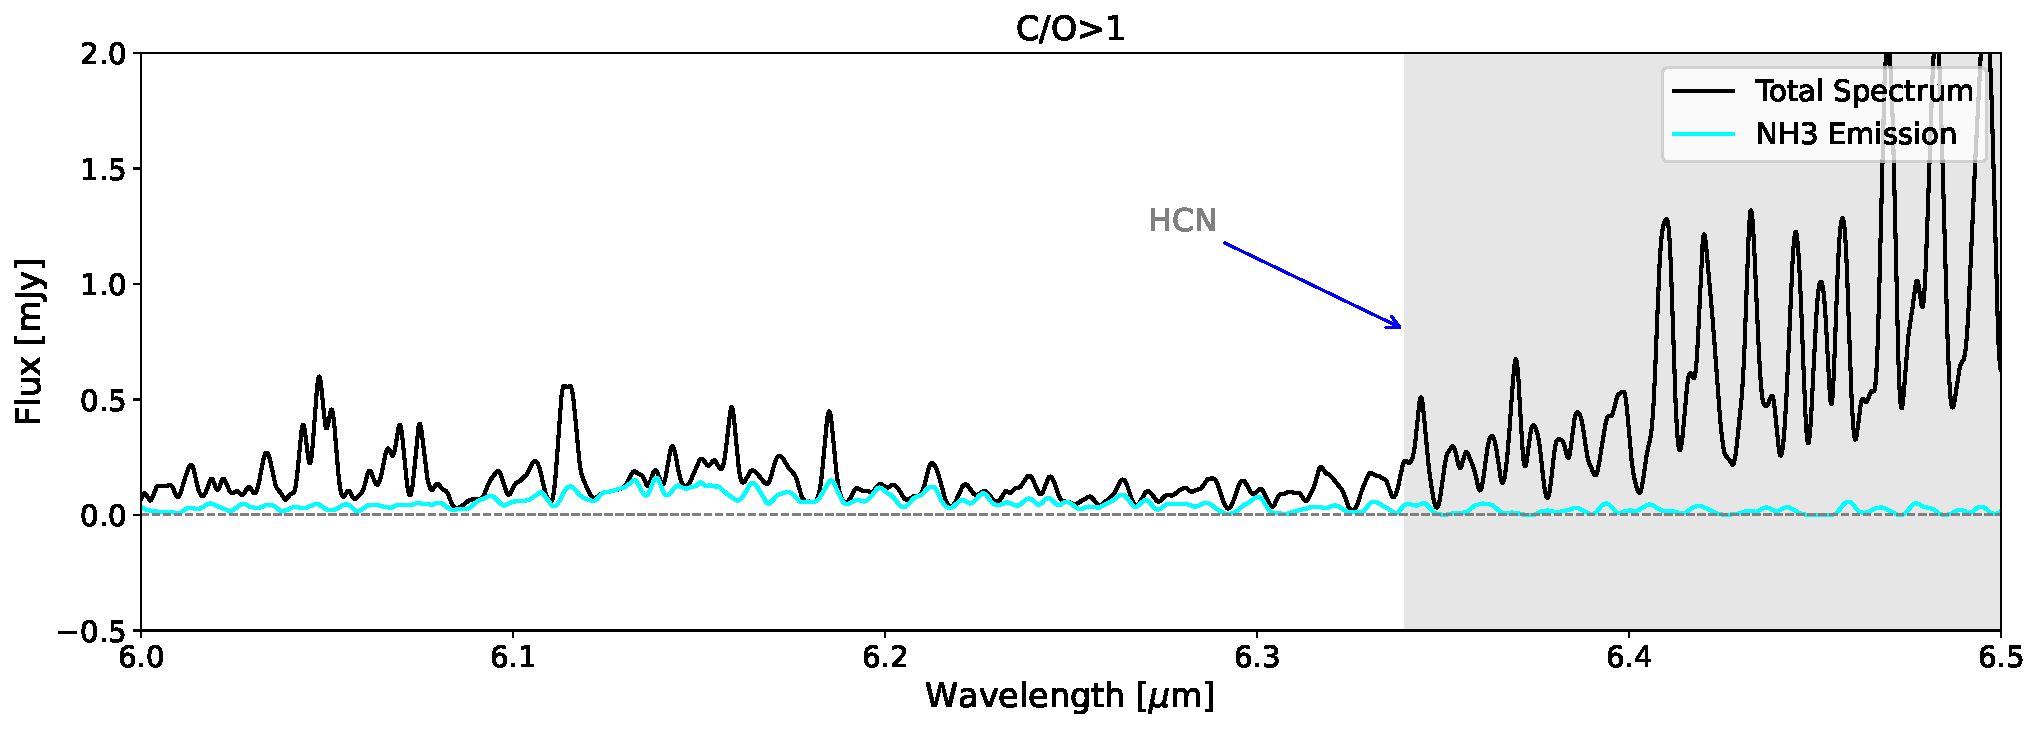
\includegraphics[width=\linewidth]{Figures/NH3_region1.pdf}
    \caption{A zoomed-in region of the spectrum of the model with C+0.25 and O-0.25 between 6 $\mu$m and 6.5 $\mu$m where NH\3 emission is strongest.}
    \label{fig: NH3 region 1}
\end{figure}
\begin{figure}[!ht]
    \centering
    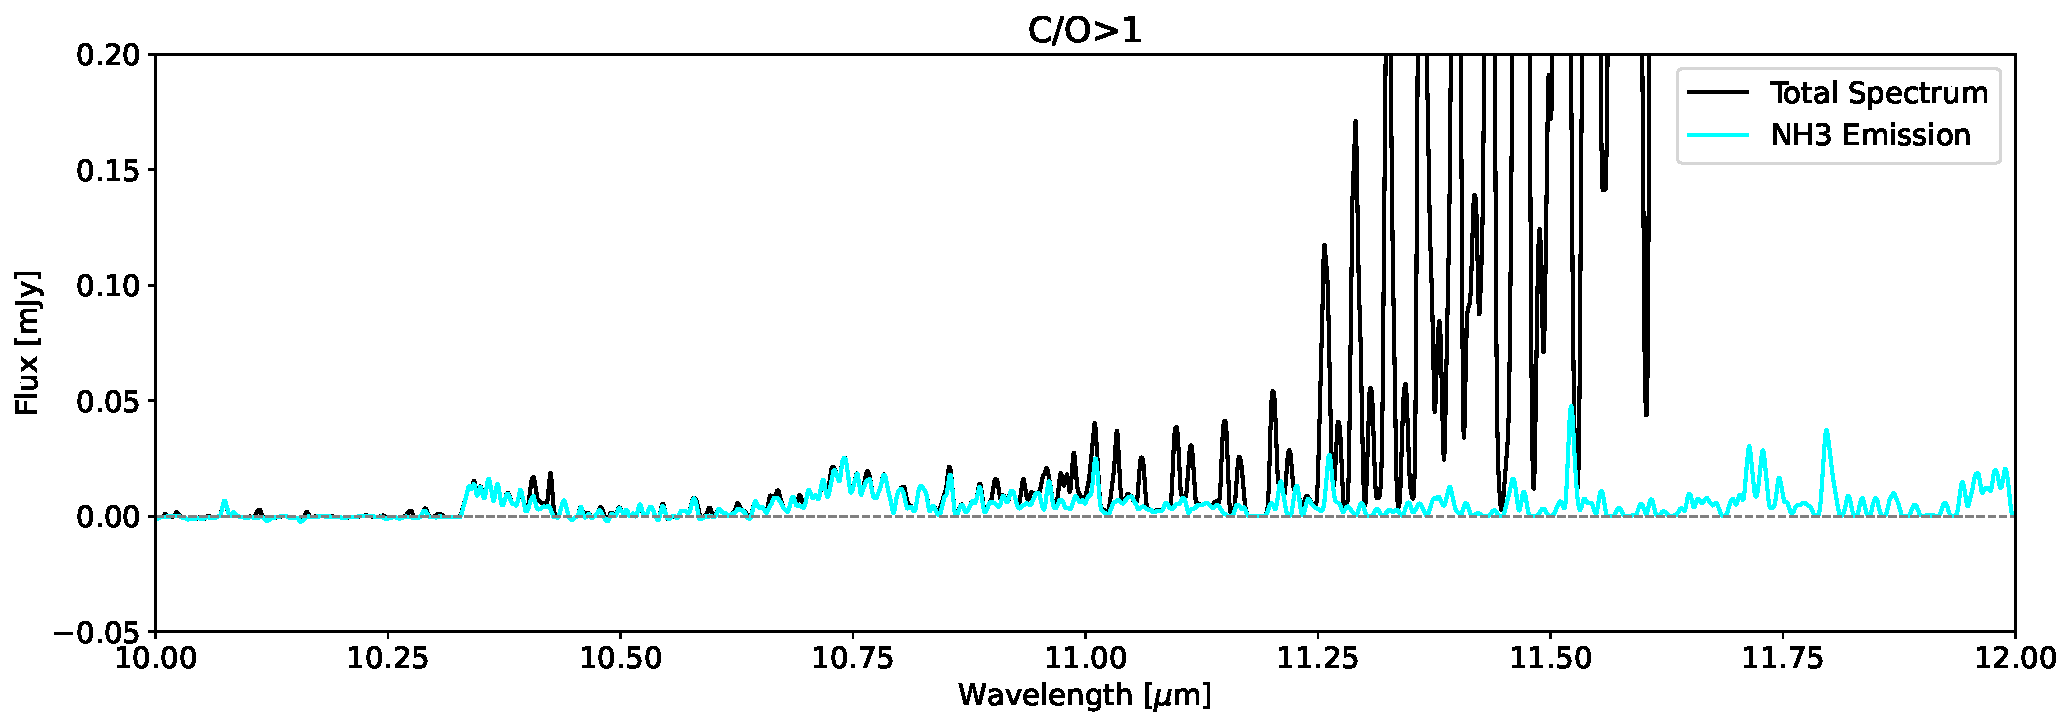
\includegraphics[width=\linewidth]{Figures/NH3_region2.pdf}
    \caption{A zoomed-in region of the spectrum of the model with C+0.25 and O-0.25 between 10 $\mu$m and 12 $\mu$m where NO emission is strongest.}
    \label{fig: NH3 region 2}
\end{figure}
\begin{figure}[!ht]
    \centering
    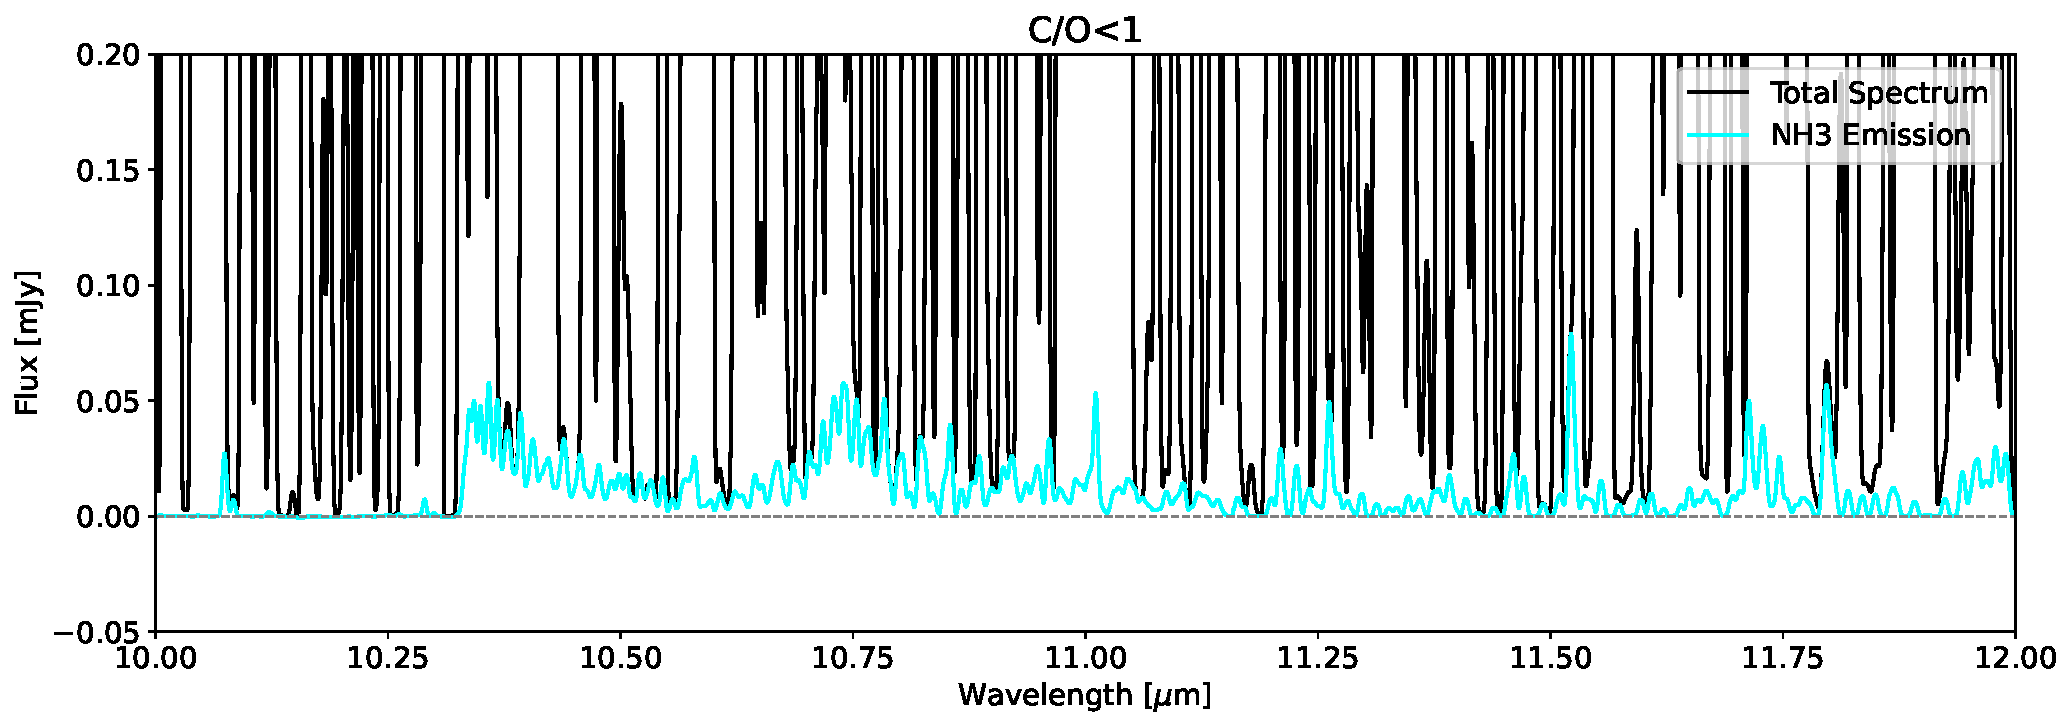
\includegraphics[width=\linewidth]{Figures/NH3_region3.pdf}
    \caption{A zoomed-in region of the spectrum of the fiducial model between 10 $\mu$m and 12 $\mu$m where NO emission is strongest.}
    \label{fig: NH3 region 3}
\end{figure}

All the spectra in figures \ref{fig: NO region}, \ref{fig: NH3 region 1}, \ref{fig: NH3 region 2}, and \ref{fig: NH3 region 3} are all without any noise. When we added noise with SNR=300 to the same spectrum shown in figure \ref{fig: NH3 region 1} based on the methods described, we got the spectrum shown in figure \ref{fig: add noise}. In this figure, the emission of NH\3 gets completely washed out in the noise, making it much more difficult to detect it.  

\begin{figure}[!ht]
    \centering
    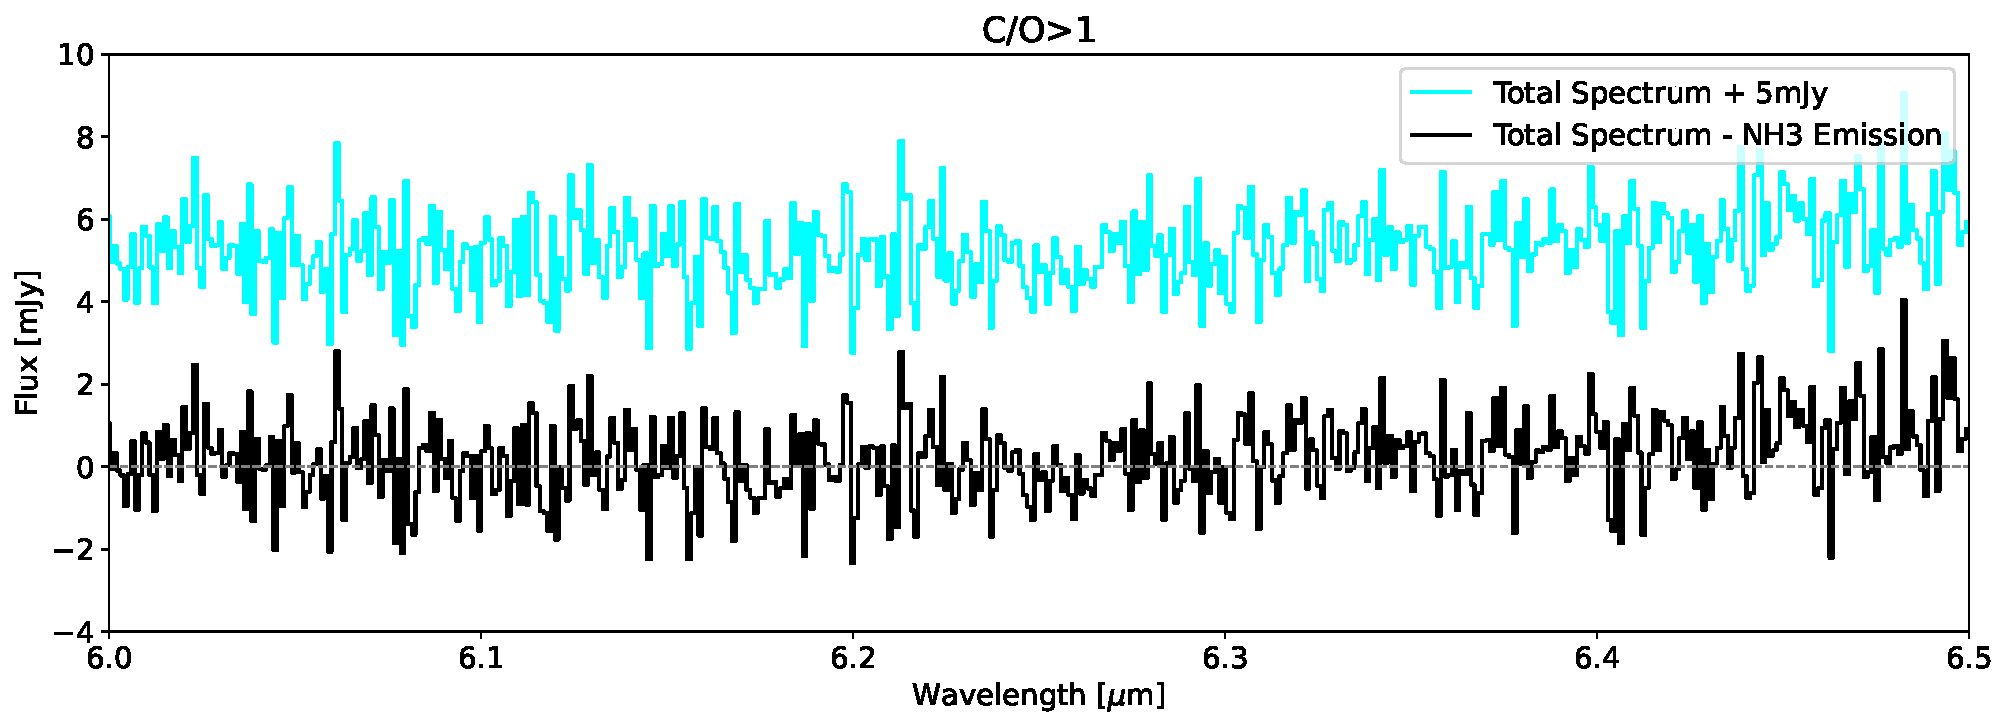
\includegraphics[width=\linewidth]{Figures/AddNoise.pdf}
    \caption{A zoomed-in region of the spectrum of the model with C+0.25 and O-0.25 between 6 $\mu$m and 6.5 $\mu$m where NH\3 emission is strongest. A Gaussian noise corresponding to an SNR of 300 is added.}
    \label{fig: add noise}
\end{figure}

\section{Molecule Detection}
As you can see in \autoref{fig: add noise}, it is hard to distinguish the NH\3 and NO from the spectrum visually. However, cross-correlation is a technique that can be used to find those weaker signals. In calculating the cross-correlation, we used the average spectrum for each species of all the models in the model grid and normalized them. This template was then used to cross-correlate with the full spectrum. In figure \ref{fig: crosscorr}, you can see the cross-correlation of the H\2O template with the spectrum of the fiducial model. The peak signals that H\2O is present in the spectrum, and it indeed is present. 

\begin{figure}[!ht]
    \centering
    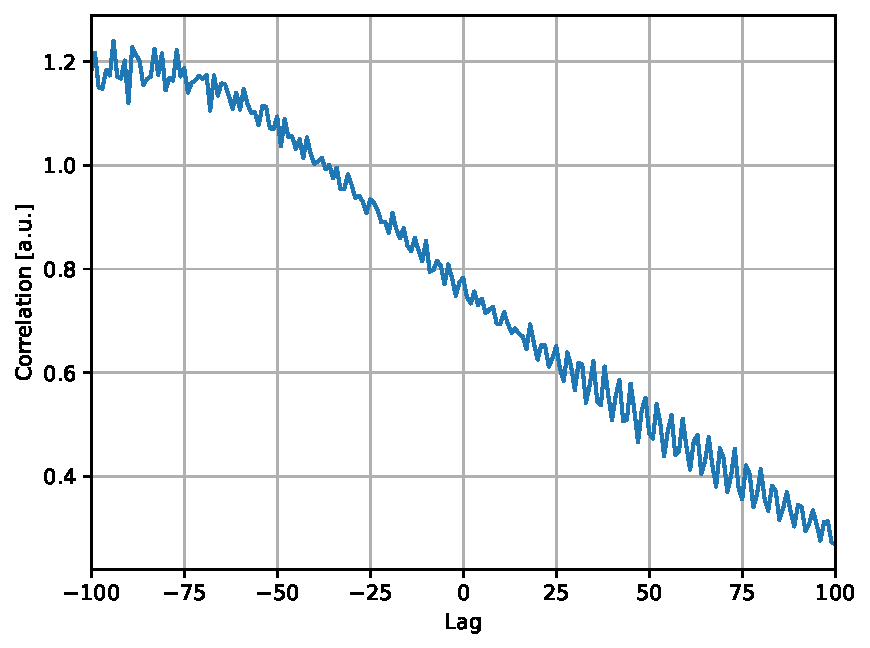
\includegraphics[width=\linewidth]{Figures/Cross-Correlation.pdf}
    \caption{The cross-correlation of the H\2O template with the spectrum the fiducial model}
    \label{fig: crosscorr}
\end{figure}

When we applied this method to the fiducial model and model C+0.25 O-0.25, we got the detections shown in table \ref{tab: fiducial detection} and \ref{tab: other detection} respectively. 

\begin{table}[!ht]
\centering
\begin{tabular}{lll}
\hline
\textbf{Molecule} & \textbf{Spectrum} & \textbf{Spectrum - Target Flux} \\ \hline
C\2H\2            & Non-detection     & Non-detection                   \\
CH\4             & Non-detection     & Non-detection                   \\
CO              & Detection         & Non-detection                   \\
CO\2             & Detection         & Non-detection                   \\
H\2O             & Detection         & Non-detection                   \\
HCN             & Non-detection     & Non-detection                   \\
NH\3             & Non-detection     & Non-detection                   \\
NO              & Non-detection     & Non-detection                   \\
OH              & Detection         & Non-detection                   \\ \hline
\end{tabular}
\caption{The detection of different molecules in the spectrum of the fiducial model using cross-correlation.}
\label{tab: fiducial detection}
\end{table}

\begin{table}[!ht]
\centering
\begin{tabular}{lll}
\hline
\textbf{Molecule} & \textbf{Spectrum} & \textbf{Spectrum - Target Flux} \\ \hline
C\2H\2            & Detection         & Non-detection                   \\
CH\4             & Non-detection     & Non-detection                   \\
CO              & Detection         & Non-detection                   \\
CO\2             & Non-detection     & Non-detection                   \\
H\2O             & Non-detection     & Non-detection                   \\
HCN             & Detection         & Non-detection                   \\
NH\3             & Non-detection     & Non-detection                   \\
NO              & Non-detection     & Non-detection                   \\
OH              & Non-detection     & Non-detection                   \\ \hline
\end{tabular}
\caption{The detection of different molecules in the spectrum of the model with C+0.25 and O-0.25 using cross-correlation.}
\label{tab: other detection}
\end{table}

We compared the cross-correlation technique for all the molecules. We did this for the spectrum of the fiducial model. Once, we cross-correlate with the spectrum to see if the molecule is present, and once with the molecule emission subtracted from the spectrum to check that this does not result in a false-positive.


% As some of the molecules have limited ranges in which they emit, we adjusted the ranges in which we cross-correlate the template and the spectrum. The ranges are listed in table \ref{}

% \begin{tabular}{lcc}
% \hline
% \textbf{Species} & \textbf{Min ($\mu$m)} & \textbf{Max ($\mu$m)} \\
% \hline
% C2H2   & 7.1 & 15.6 \\
% CH4    & 6.3 & 9.7 \\
% CO     & 4.9 & 5.6 \\
% CO2    & 13.0 & 17.3 \\
% H2O    & 4.9 & 27.5 \\
% HCN    & 6.4 & 17.0 \\
% NH3    & 5.1 & 27.5 \\
% NO     & 4.9 & 6.6 \\
% OH     & 8.3 & 27.5 \\
% \hline
% \end{tabular}



% Using the ranges in table \ref{}. We redid our analysis and got the following.

% \textbf{INSERT TABLE OF DETECTION PARTIAL RANGE}

As some of the flux of a species overlaps with the flux emitted by other species, it would make detection easier if the flux of the other species were removed. This was easily done with the simulated data, as the simulation gave the spectra of the individual species. Especially the region where NO is emitted is of interest, as the only other species that emit in that range are CO and H\2O. Removing the flux of CO and H\2O for the fiducial gave the spectrum shown in figure \ref{fig: H2O and CO removed}

\begin{figure}
    \centering
    \includegraphics[width=0.5\linewidth]{Fiducial H2O and CO removed}
    \caption{A zoomed-in region of the spectrum of the fiducial model between 4.9 $\mu$m and 6 $\mu$m. The emission of both H\2O and CO has been removed.}
    \label{fig: H2O and CO removed}
\end{figure}

\section{Application on Observations}
We applied the techniques of the previous part to real data to see if they are effective here as well

We cross-correlated the templates with the measured spectra. The results of this are shown in table \ref{tab: realdata}.

\begin{table}[!ht]
\centering
\begin{tabular}{llll}
\hline
\textbf{Specie} & \textbf{GWLup} & \textbf{Sz98} & \textbf{V1094Sco} \\ \hline
C2H2            & Detection      & Non-detection & Detection         \\
CH4             & Non-detection  & Non-detection & Non-detection     \\
CO              & Detection      & Detection     & Detection         \\
CO2             & Detection      & Detection     & Detection         \\
H2O             & Detection      & Detection     & Detection         \\
HCN             & Detection      & Detection     & Detection         \\
NH3             & Non-detection  & Non-detection & Non-detection     \\
NO              & Non-detection  & Non-detection & Non-detection     \\
OH              & Detection      & Detection     & Detection         \\ \hline
\end{tabular}
\caption{The detection of different molecules in the spectra of GWLup, Sz98, and V1094Sco using cross-correlation.}
\label{tab: realdata}
\end{table}


We used 1D LTE models to fit CO and H\2O in the region 4.9-6.5 $\mu$m.

\begin{figure}[!ht]
    \centering
    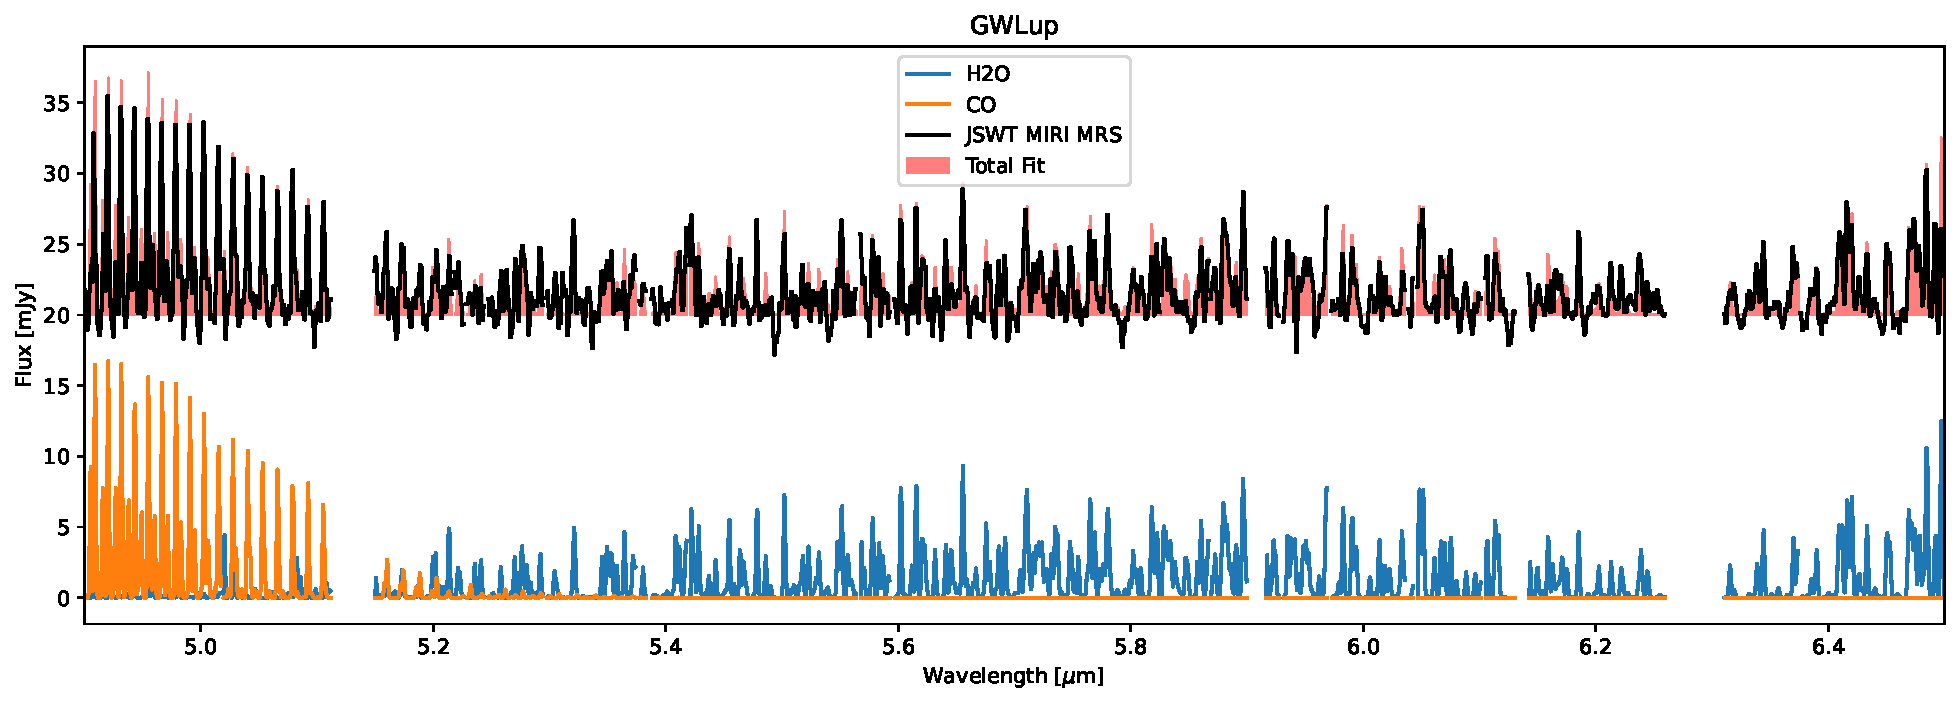
\includegraphics[width=\linewidth]{Figures/Fit_GWLup.pdf}
    \caption{The fitted H\2O and CO spectra using a 1D LTE model between 4.9 $\mu$m and 6.5$\mu$m for GWLup}
    \label{fig: fit gwlup}
\end{figure}
\begin{figure}[!ht]
    \centering
    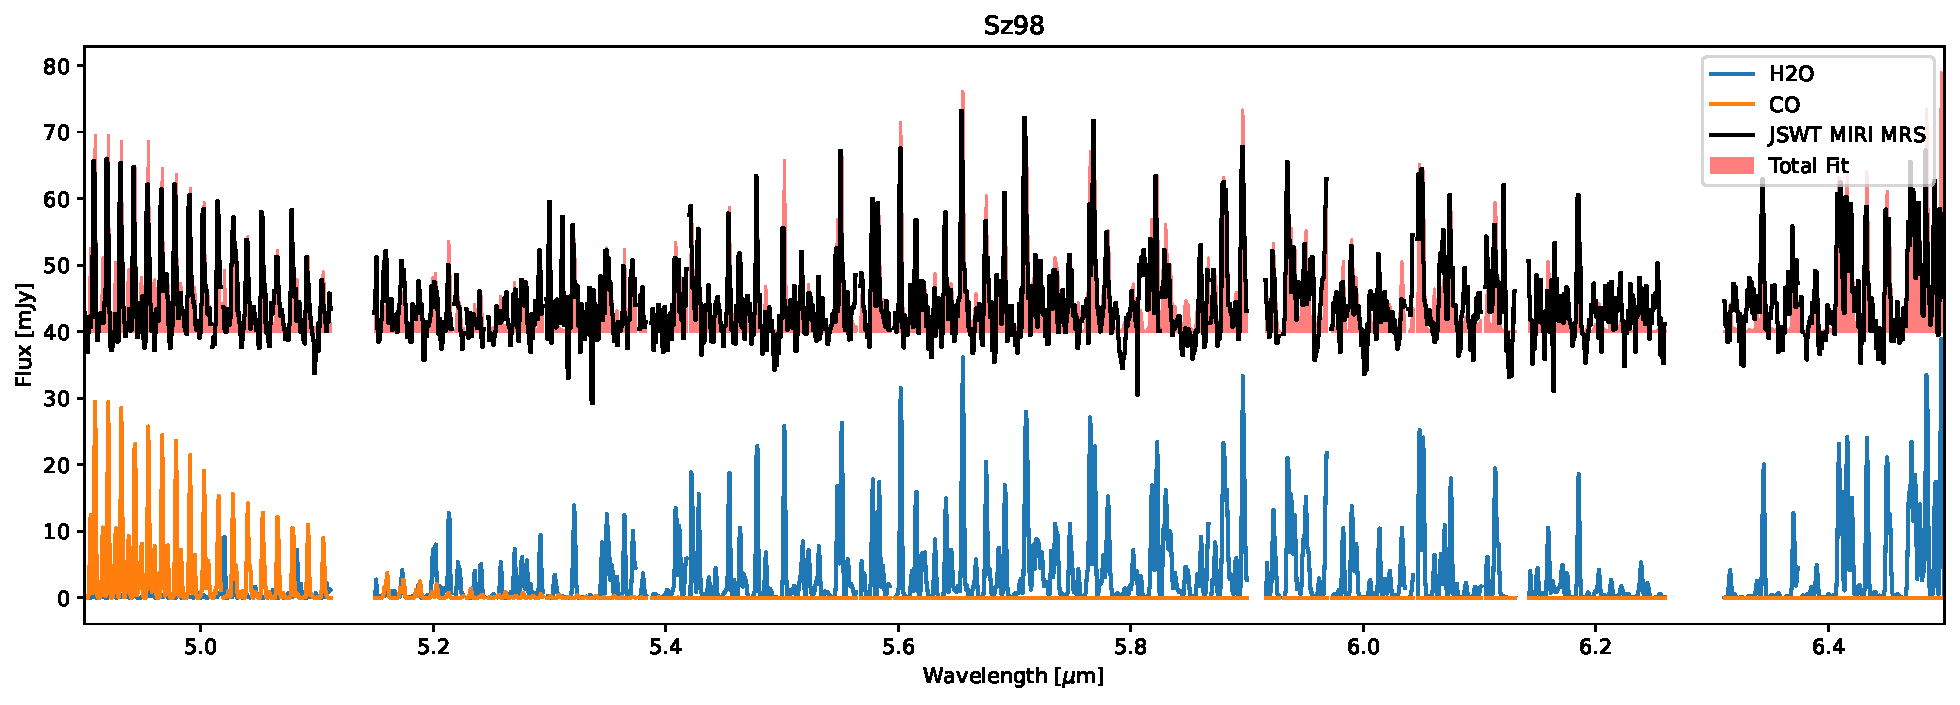
\includegraphics[width=\linewidth]{Figures/Fit_Sz98.pdf}
    \caption{The fitted H\2O and CO spectra using a 1D LTE model between 4.9 $\mu$m and 6.5$\mu$m for Sz98}
    \label{fig: fit sz98}
\end{figure}
\begin{figure}[!ht]
    \centering
    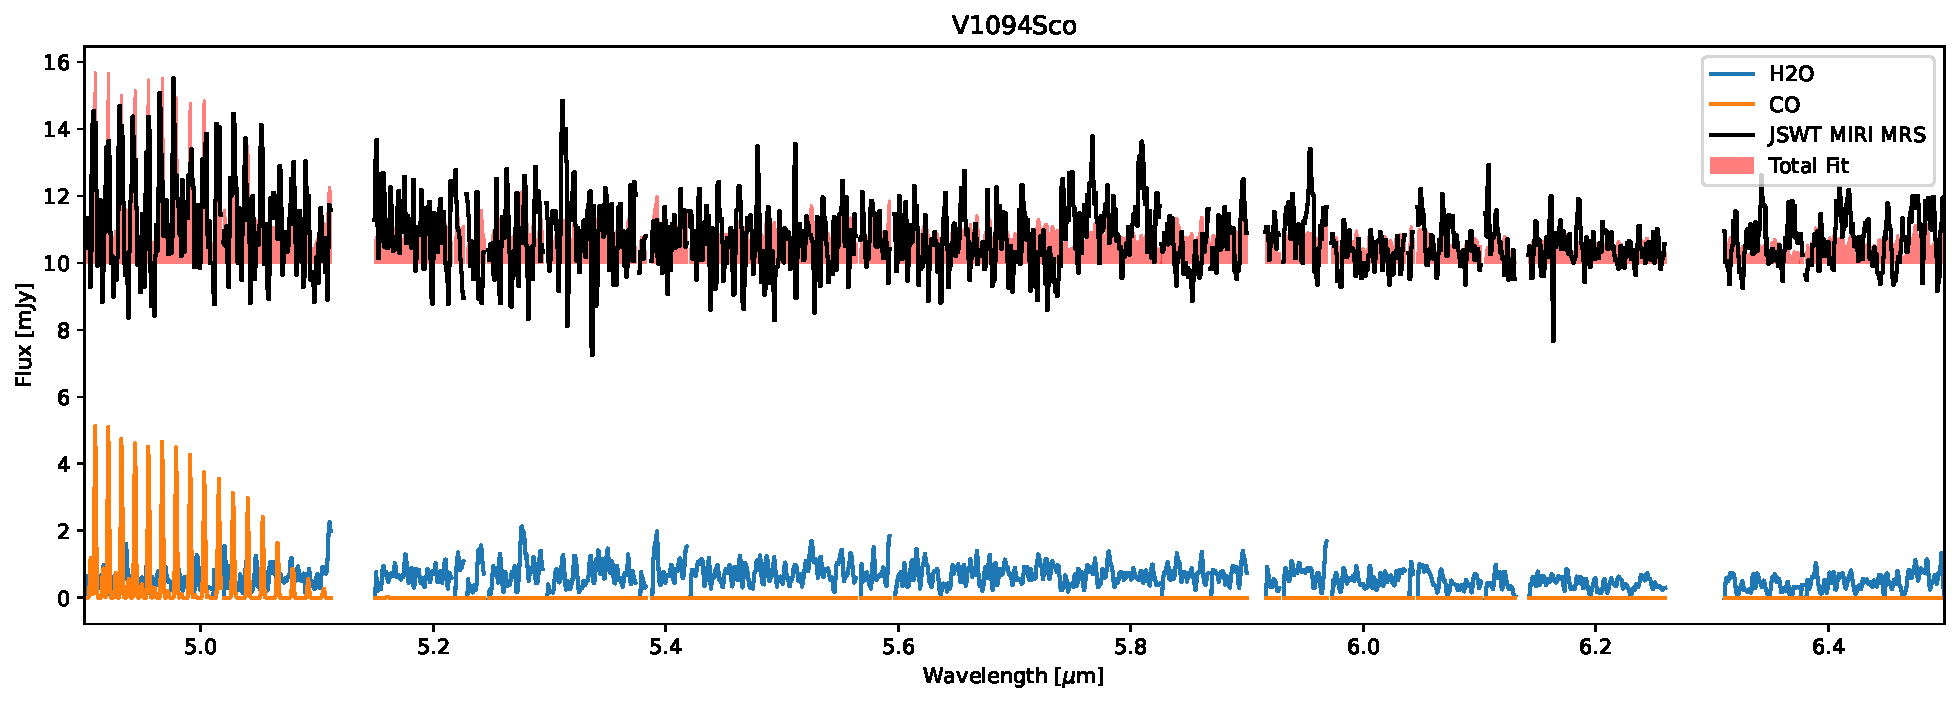
\includegraphics[width=\linewidth]{Figures/Fit_V1094Sco.pdf}
    \caption{The fitted H\2O and CO spectra using a 1D LTE model between 4.9 $\mu$m and 6.5$\mu$m for V1094Sco}
    \label{fig: v1094sco}
\end{figure}

After removing the fits from the spectra and redoing the cross-correlation, we detected NO emission in the spectrum of V1094Sco.

\chapter{Discussion}\label{Ch: Discussion}
\section{Interpretation}
\section{Comparison to Other Works}
\cite{Grant_2023} have detected CO, CO\2, H\2O, HCN, C\2H\2 and OH in the spectrum of GWLup. These are the same molecules we detected using our cross-technique. In the spectrum of Sz98 \cite{Gasman_2023} have detected CO, H\2O, OH, CO\2, and HCN. These are again the same molecules we detected. The fact that we have the same results as them, is a promising sign for the validity of our technique. 
\section{Limitations}
Assumptions:

- average noise=0

- center peak can come from other sources

- bootstrapping of fluxes

- averaging of the emission of each species

\section{Future Work}


\chapter{Conclusion}\label{Ch: Conclusion}

\bibliographystyle{aa.bst}
\bibliography{references}
\end{document}